%!TEX root = ../template.tex
%%%%%%%%%%%%%%%%%%%%%%%%%%%%%%%%%%%%%%%%%%%%%%%%%%%%%%%%%%%%%%%%%%%
%% chapter4.tex
%% NOVA thesis document file
%%
%% Chapter 4: Technological Implementation
%%%%%%%%%%%%%%%%%%%%%%%%%%%%%%%%%%%%%%%%%%%%%%%%%%%%%%%%%%%%%%%%%%%

\typeout{NT FILE chapter4.tex}%

\chapter{Technological Implementation}
\label{cha:implementation}

This chapter describes how the \gls{DT} framework from \Cref{cha:architecture} was implemented in practice. Moving from conceptual designs to a working system requires connecting standardized semantic models, such as the \gls{AAS}, with game-engine physics, interactive software tools, and industrial shop-floor hardware.

To evaluate the pipeline under realistic manufacturing conditions, each layer was implemented and tested on a physical modular \gls{FMS} bench.

The chapter is organized as follows:
\begin{itemize}
    \item \Cref{sec:tech_realization} introduces the physical \gls{FMS} bench and gives an overview of the global component architecture and its interfaces.
    \item \Cref{sec:impl_layer0} presents Layer~0 (Physical Asset Digitization), covering physical measurements, low-polygon 3D modeling, pivot rigging, and \gls{GLB} export in Blender.
    \item \Cref{sec:impl_wizard} describes Layer~1 (Asset Modeling), detailing the PyQt6 and PyVista desktop application, the binding of sensors and actuators to model nodes, the no-code control logic editor, and \gls{AASX} package generation with the BaSyx Python \gls{SDK}.
    \item \Cref{sec:impl_basyx} covers Layer~2 (Storage and Registry), explaining the containerized Eclipse BaSyx~v2 microservices, port mappings, and MongoDB database.
    \item \Cref{sec:impl_unity} details Layer~3 (Runtime Execution and Physical Synchronization), focusing on procedural scene assembly in Unity 3D, PhysX contact mechanics, dual-mode execution (\gls{VC} and operational \gls{DT}), and kinematic drift correction.
    \item \Cref{sec:impl_firmware} describes the physical automation setup and embedded firmware running FreeRTOS on an Industrial Shields M-DUINO \gls{PLC}, including sensor scanning, low-latency \gls{TCP} telemetry, and \gls{HTTP} actuation.
    \item \Cref{sec:impl_traceability} maps each technical component to its functional and non-functional requirements in a traceability matrix.
\end{itemize}

\section{System Architecture and Technology Realization}
\label{sec:tech_realization}

Turning the conceptual architecture from \Cref{cha:architecture} into a working implementation requires matching abstract layer roles to concrete software tools, network protocols, and hardware platforms. This section describes the modular \gls{FMS} bench used for testing and outlines the overall component architecture.

\subsection{Physical Testbed Context: The Modular \texorpdfstring{\gls{FMS}}{FMS} Bench}
To validate the framework, an existing \gls{FMS} testbed was used as the pilot case study (\Cref{fig:fms_pilot_testbed}), based on the modular \gls{CPPS} architecture proposed by \textcite{Rocha2024}. The physical apparatus is an educational and industrial training model built using \textit{fischertechnik} modular mechatronic components, organized as a closed-loop conveyor bench to transport pallets across processing and inspection stations. While compact in physical footprint, this testbed replicates the electromechanical topology and real-time control constraints of real-world production cells, making it well-suited to evaluate whether the \gls{DT} can reconstruct a factory floor modularly, asset by asset, and coordinate distributed mechanisms in real time.

\begin{figure}[htbp]
    \centering
    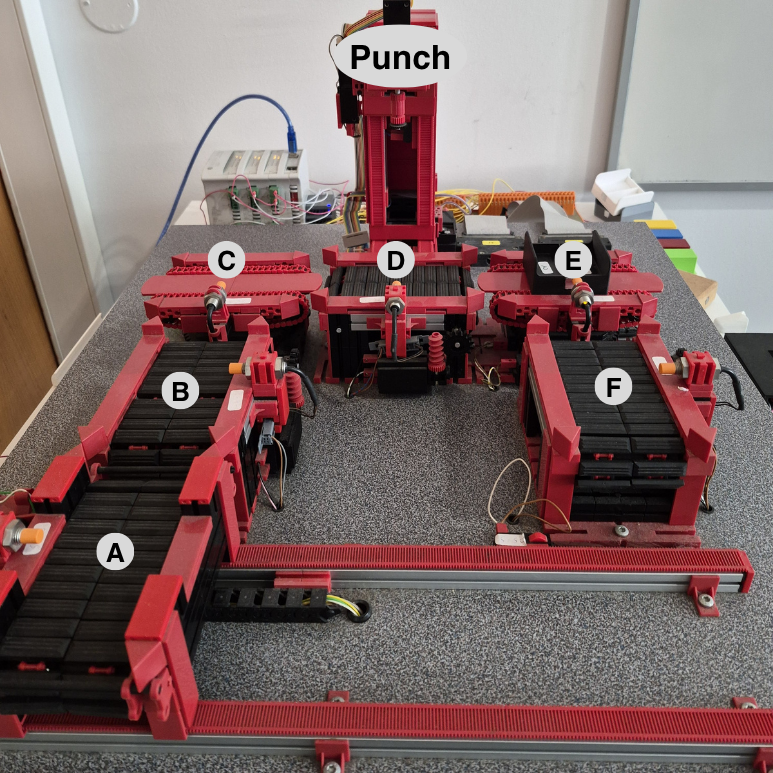
\includegraphics[width=0.72\linewidth,height=0.42\textheight,keepaspectratio]{5-Figures/fms_pilot_bench.jpg}
    \caption{Physical modular \gls{FMS} conveyor testbed built with fischertechnik mechatronic modules, showing the conveyor tracks, magnetic sensors, punch mechanism, and Industrial Shields M-DUINO \gls{PLC}.}
    \label{fig:fms_pilot_testbed}
\end{figure}

Mechanically, the bench includes three stationary conveyor belts (Conveyors B, D, and F), two rotating sections (Conveyors C and E), one translating conveyor (Conveyor A), and a punch mechanism that simulates drilling, stamping, or screwing operations. Field instrumentation consists of 24\,V~DC magnetic track sensors to detect workpieces, contact limit switches to monitor conveyor and punch positions, and 24\,V~DC motors driving each section. Control is managed by an Industrial Shields M-DUINO 57R+ \gls{PLC} (based on the Arduino Mega 2560), equipped with an Ethernet port and optocoupled \gls{IO} boards. Digital input pins (I0\_0 to I2\_3) read sensor states, while relay outputs (R0\_2 to R2\_8) command conveyor motors and punch actions (the full pin assignment is listed in \Cref{app:fms_io_mapping}).

\subsection{Overall Component Architecture and Inter-Layer Interfaces}
With this physical bench as the target, the complete framework was implemented across four operational layers. The \gls{UML} Component Diagram in \Cref{fig:architecture_global} illustrates the overall system implementation architecture across the four operational layers.

\begin{figure}[htbp]
    \centering
    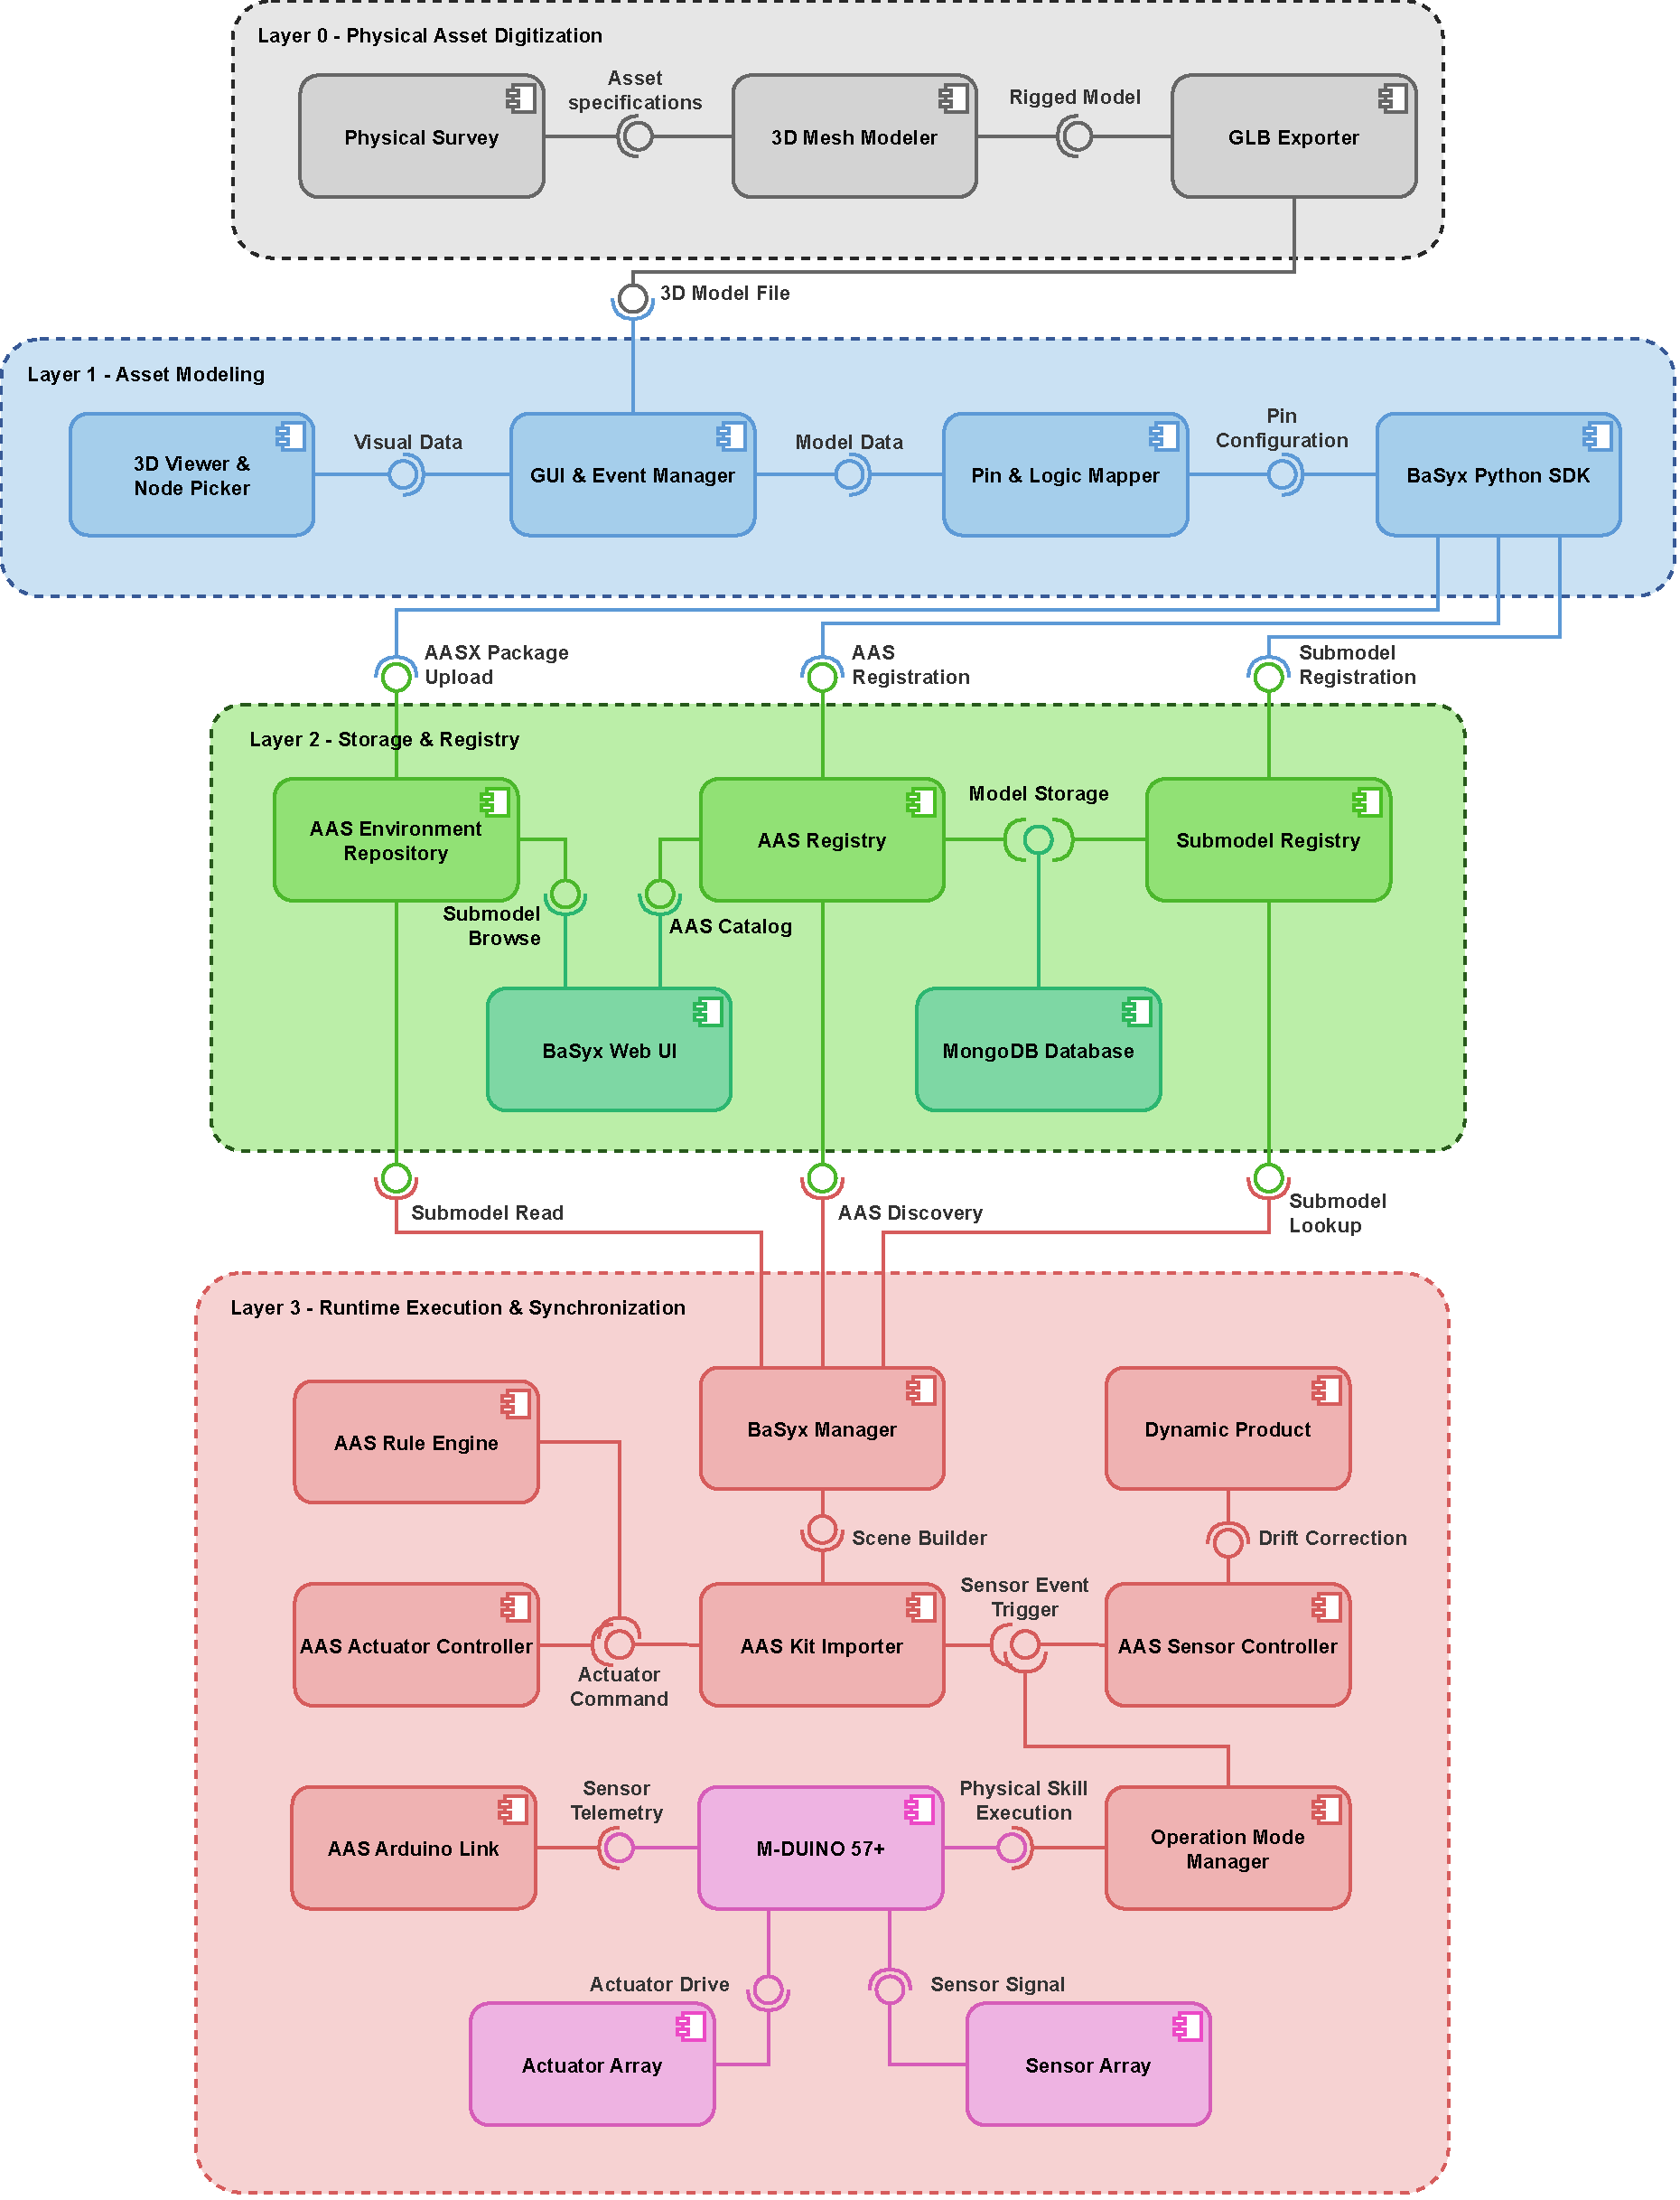
\includegraphics[width=\textwidth]{5-Figures/Implementação.drawio.pdf}
    \caption[\gls{UML} Component Diagram of the framework implementation architecture]{\gls{UML} Component Diagram of the framework implementation architecture: (0) Physical Asset Digitization in Blender, (1) Asset Modeling in the Python desktop application, (2) Storage and Registry in Eclipse BaSyx~v2 on Docker, and (3) Runtime Execution and Physical Synchronization in Unity 3D with an Industrial Shields M-DUINO \gls{PLC}.}
    \label{fig:architecture_global}
\end{figure}

The information flow spans four operational stages. In Layer~0 (Physical Asset Digitization), physical hardware components are rebuilt as 3D models in Blender using manual measurements. These models are rigged with pivot axes and sensor colliders, then exported as binary \gls{glTF} files (.glb). Next, Layer~1 (Asset Modeling) runs as a desktop application that loads the 3D model into an interactive viewport. Here, users configure machine properties and assign \gls{IO} pins before the BaSyx Python \gls{SDK} packages everything into an \gls{AASX} bundle and uploads it to Layer~2 via \gls{REST} endpoints. 

In Layer~2 (Storage and Registry), Eclipse BaSyx~v2 services run inside Docker containers. An \gls{AAS} Environment Repository stores package files, while the \gls{AAS} Registry and Submodel Registry track active assets and submodel URLs backed by MongoDB. Operators can inspect these assets through the BaSyx Web \gls{GUI}. Finally, Layer~3 (Runtime Execution and Physical Synchronization) runs the 3D simulation in Unity, connecting directly to the physical testbed controlled by the Industrial Shields M-DUINO \gls{PLC}. At startup, Unity queries BaSyx to retrieve models and assemble the scene automatically. During operation, the runtime either runs in \gls{VC} mode using local rules or synchronizes live with physical hardware by exchanging low-latency \gls{TCP} telemetry and \gls{HTTP} commands with the \gls{PLC}.

\section{Layer 0: Physical Asset Digitization and 3D Modeling}
\label{sec:impl_layer0}
\label{subsec:layer0_modeling}

As established in \Cref{sec:layer0_conceptual} (\cpageref{sec:layer0_conceptual}), physical machinery on existing factory floors often lacks simulation-ready 3D models. When manufacturing \gls{CAD} files do exist, their high polygon count slows down real-time physics engines, while missing functional motion joints, pivot points, and interaction colliders. Because the modular \gls{FMS} bench had no existing vendor models, Layer~0 was carried out as an upstream preparatory stage in Blender 5.2.0 LTS to create lightweight, rigged \gls{GLB} assets.

The \gls{UML} Component Diagram in \Cref{fig:component_layer0} illustrates the component architecture of Layer~0, structured into three sequential tasks:
\begin{enumerate}
    \item \textbf{Physical Measurements:} Measuring the dimensions of the physical \gls{FMS} modules using a measuring tape.
    \item \textbf{3D Mesh Modeling and Kinematic Rigging:} Reconstructing modules at a 1:1 scale matching Unity's coordinate frame.
    \item \textbf{\gls{GLB} Packaging:} Exporting self-contained binary \gls{glTF} files (.glb) containing geometry, materials, hierarchies, and trigger colliders for direct ingestion into Layer~1.
\end{enumerate}

\begin{figure}[htbp]
    \centering
    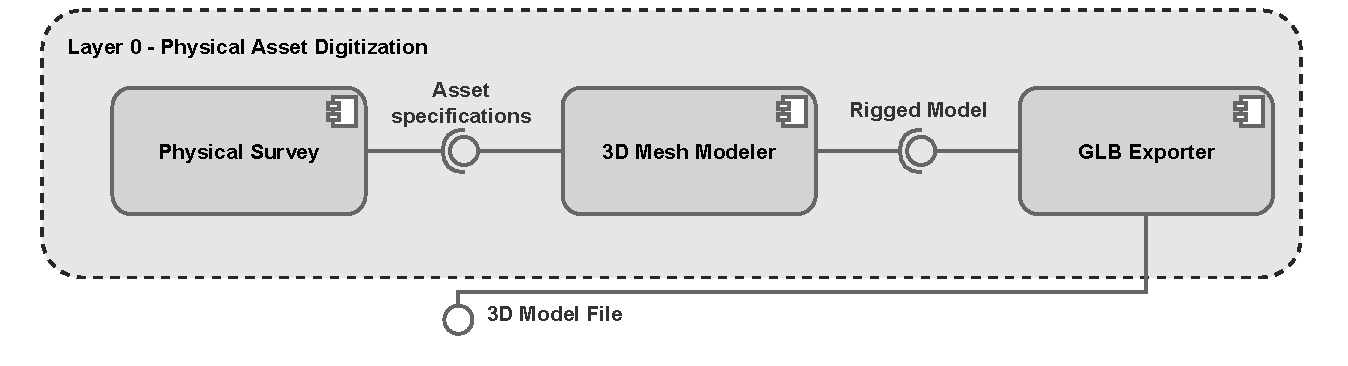
\includegraphics[width=\linewidth,height=0.72\textheight,keepaspectratio]{5-Figures/Layer 0 - Physical Asset Digitization.pdf}
    \caption{\gls{UML} Component Diagram of Layer 0 (Physical Asset Digitization).}
    \label{fig:component_layer0}
\end{figure}

\begin{figure}[htbp]
    \centering
    \begin{subfigure}[t]{0.48\textwidth}
        \centering
        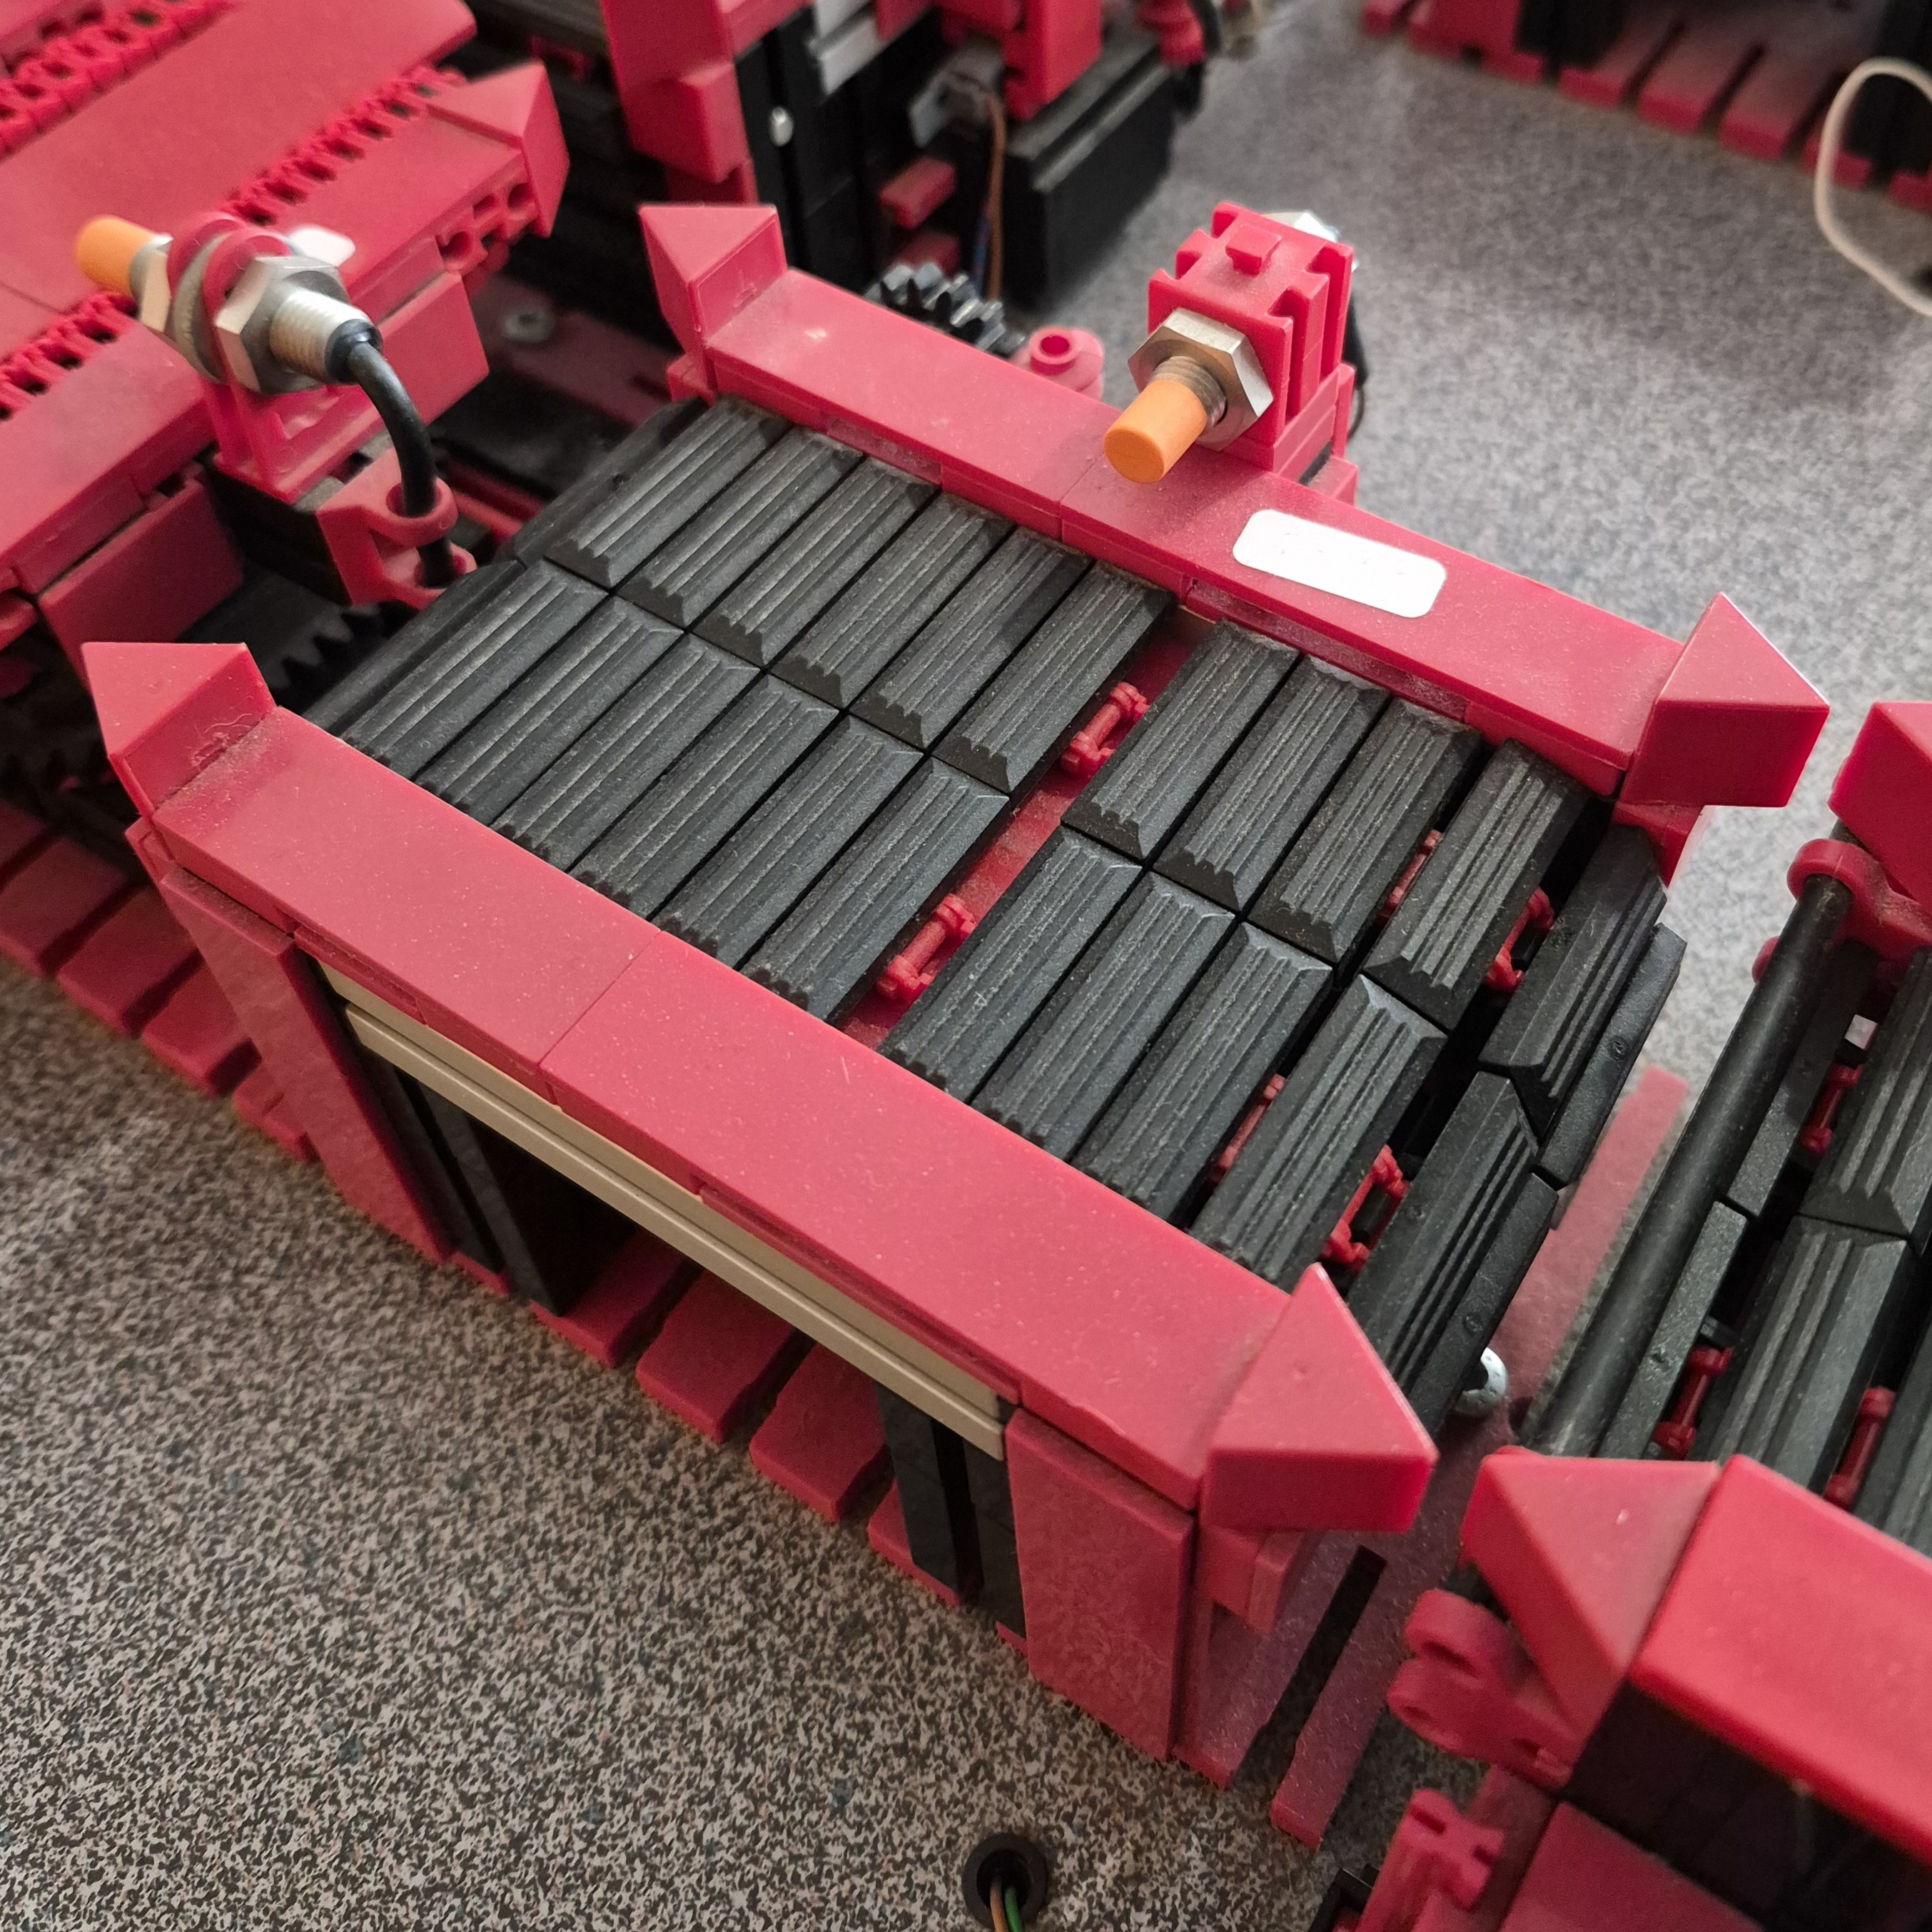
\includegraphics[width=\linewidth,height=5.8cm,keepaspectratio]{5-Figures/fms_conveyor_sensors_closeup.jpg}
        \caption{Physical conveyor module.}
        \label{fig:fms_physical_module}
    \end{subfigure}
    \hfill
    \begin{subfigure}[t]{0.48\textwidth}
        \centering
        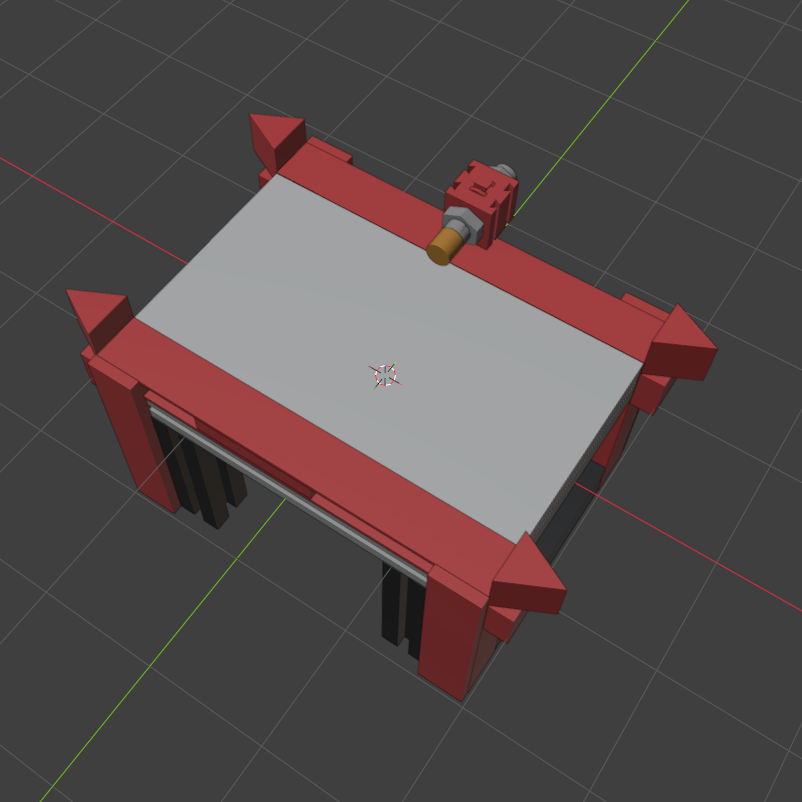
\includegraphics[width=\linewidth,height=5.8cm,keepaspectratio]{5-Figures/blender_kLfhitpziL.png}
        \caption{Reconstructed 3D asset.}
        \label{fig:blender_3d_module}
    \end{subfigure}
    \caption{Comparison between the physical modular \gls{FMS} conveyor module and its reconstructed 3D simulation model in Blender.}
    \label{fig:fms_physical_vs_blender}
\end{figure}

To meet the requirements of the \textit{VisualStructure} metamodel (\Cref{sec:model_visual_structure}, \cpageref{sec:model_visual_structure}), each asset was structured into a clean parent-child hierarchy separating static frames from moving mechanisms. Static chassis parts were merged into a single root node with its coordinate origin set at the base reference point $(0, 0, 0)$. Dynamic elements, such as conveyor belts, rotating conveyors, and the punch station, were isolated into child objects. 

The pivot point of each moving component was aligned with its physical axis of rotation or linear motion vector. In physics engines, an offset pivot causes parts to rotate or translate along unintended paths when animated by \textit{BehaviorBinding} scripts (\Cref{sec:model_behavior_mapping}, \cpageref{sec:model_behavior_mapping}). In addition, invisible geometric trigger colliders were placed at physical sensor locations to detect passing workpieces during simulation. Once modeled and validated, all modules were exported as compact binary \gls{GLB} files ready for the modeling application.


\section{Layer 1: Asset Modeling Desktop Application}
\label{sec:impl_wizard}

Layer~1 was implemented as a standalone desktop application. It combines the Asset Model Editor and Package Exporter roles from \Cref{sec:layer1_conceptual} (\cpageref{sec:layer1_conceptual}) into a single tool. In line with requirement \textbf{NFR4} (Configuration Accessibility), the goal was to allow engineers to configure a \gls{DT} asset without writing any code.

The \gls{UML} Component Diagram in \Cref{fig:component_layer1} shows the component structure of Layer~1 (Asset Modeling), divided into four modules: (1) the 3D Viewer renders the model and detects which mesh node the user clicks, (2) the \gls{GUI} \& Event Manager provides the PyQt6 interface with step-by-step tabs, (3) the Pin \& Logic Mapper links visual sensor placements and kinematic rules to controller pin registers, and (4) the BaSyx Python \gls{SDK} builds the in-memory \gls{AAS} submodels, packages the \gls{AASX} archive, and uploads it to Layer~2 via \gls{REST} endpoints.

\begin{figure}[htbp]
    \centering
    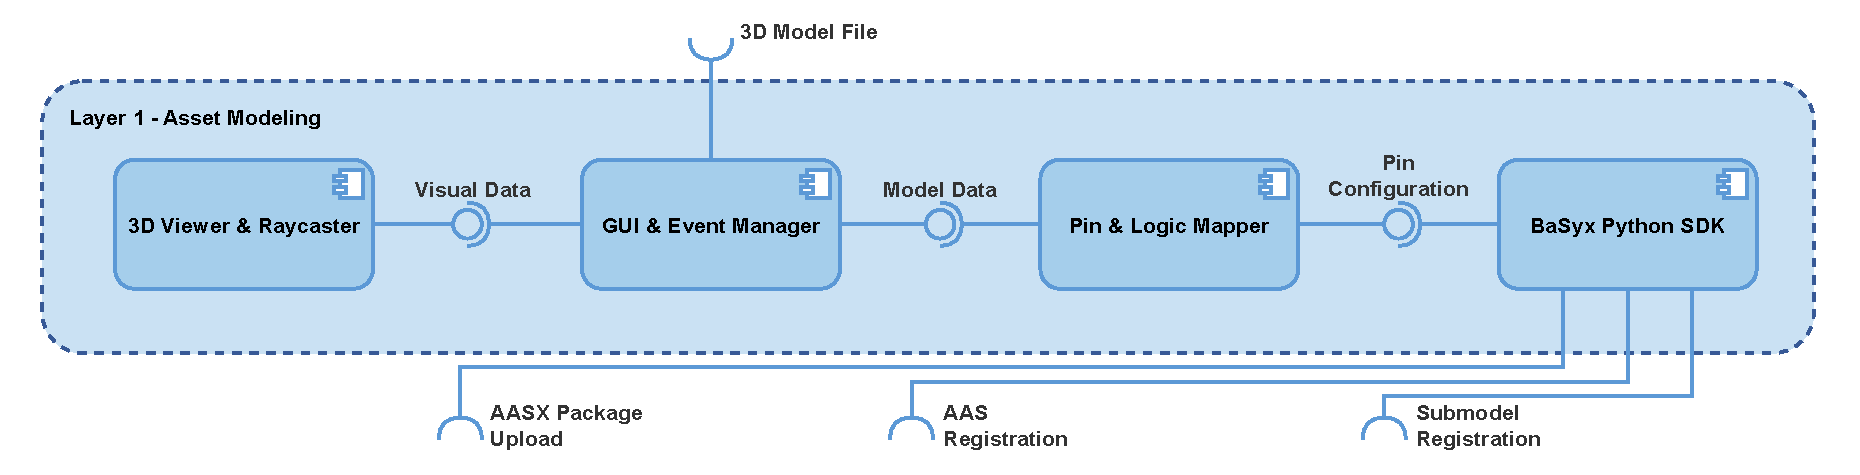
\includegraphics[width=\linewidth,height=0.72\textheight,keepaspectratio]{5-Figures/Layer 1 - Asset Modeling.pdf}
    \caption{\gls{UML} Component Diagram of Layer 1 (Asset Modeling).}
    \label{fig:component_layer1}
\end{figure}

\subsection{\texorpdfstring{\gls{AAS}}{AAS} Data Model \& Submodel Specifications}
Rather than following a rigid sequence, the modeling tool acts as an editor that populates standardized \gls{IEC}~63278 \gls{AAS} submodels (\Cref{fig:asset_metamodel_conceptual}, \cpageref{fig:asset_metamodel_conceptual}). Although the \gls{IDTA} provides official templates for static equipment data (such as \textit{Digital Nameplate}), it lacks standard definitions for 3D physics, spatial sensor placement, and live controller synchronization.

To fill this gap, the tool implements the domain-specific submodels defined in \Cref{sec:asset_data_model} (\cpageref{sec:asset_data_model}):
\begin{itemize}
    \item \textbf{\textit{VisualStructure}}: Stores the 3D \gls{GLB} file and defines the transform hierarchy (position, rotation, scale) for rendering.
    \item \textbf{\textit{VirtualPins}}: Maps sensors and actuators to physical \gls{PLC} addresses (such as \texttt{I0\_0} or \texttt{R0\_2}) and stores their boolean values.
    \item \textbf{\textit{BehaviorMapping}}: Binds components to motion parameters, defining translation or rotation axes, continuous speeds, and sensor trigger envelopes.
    \item \textbf{\textit{AssetInterfacesDescription}} (or \textbf{\textit{NetworkEndpoint}}): Configures network communication settings, including controller \gls{IP} addresses, ports, and protocol bindings.
    \item \textbf{\textit{ControlLogic}}: Formats IF-THEN rules into structured conditions for local edge execution during \gls{VC}.
\end{itemize}

\subsection{Modeling Tool \texorpdfstring{\gls{GUI}}{GUI} and 3D Viewport Architecture}
The desktop application is built with PyQt6, providing a graphical interface that avoids writing raw \gls{JSON} files by hand. The central 3D viewport uses PyVista and \gls{VTK}, with Trimesh handling geometry operations. Within the viewport, users can inspect bounding dimensions and navigate the mesh hierarchy (\Cref{fig:conveyor_wizard_gui_screenshot}).

\begin{figure}[htbp]
    \centering
    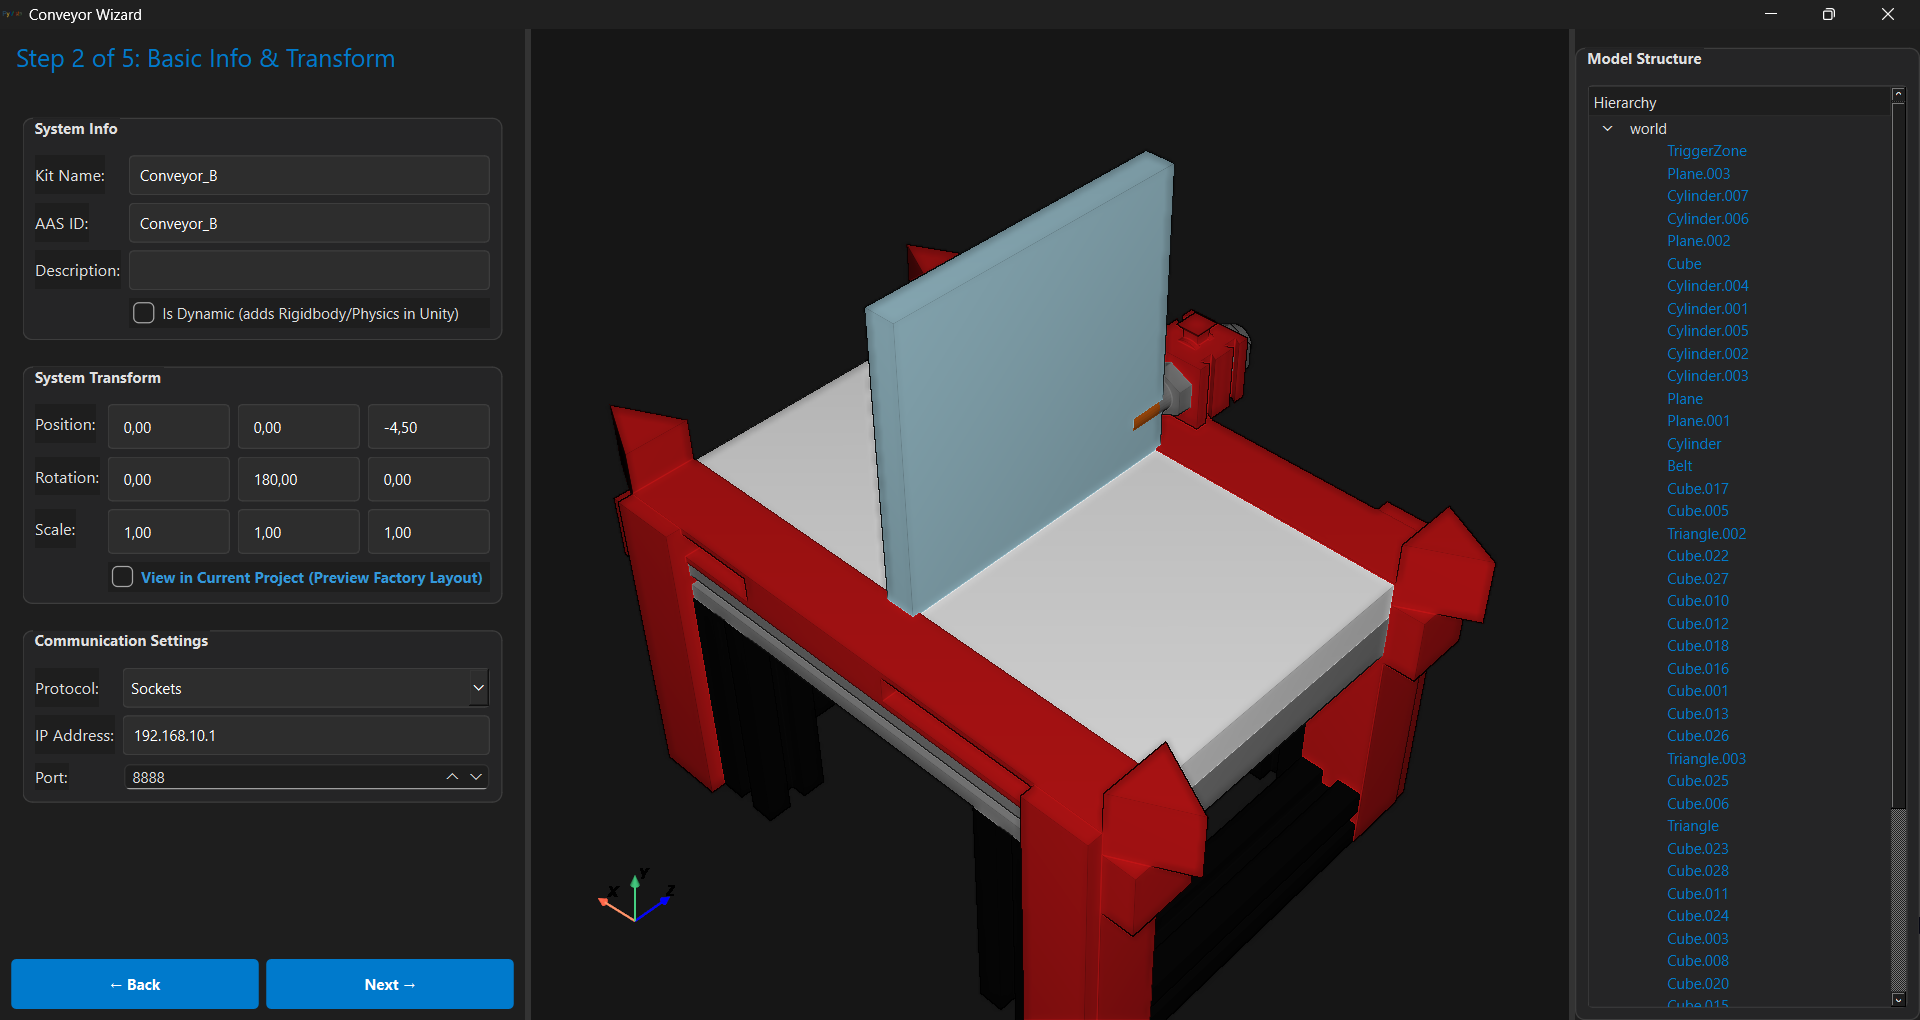
\includegraphics[width=\linewidth,keepaspectratio]{5-Figures/asset_modeling_gui.png}
    \caption{\gls{GUI} of the Asset Modeling application showing the interactive 3D viewport, configuration panels, and model structure hierarchy.}
    \label{fig:conveyor_wizard_gui_screenshot}
\end{figure}

As shown in \Cref{fig:conveyor_wizard_gui_screenshot}, the interface is divided into three main sections:
\begin{itemize}
    \item \textbf{Interactive 3D Viewport (Center):} Displays the 3D model with camera controls (orbit and pan) and visual markers for placed pins and coordinate axes.
    \item \textbf{Configuration Wizard (Left Panel):} Guides the engineer through five sequential setup tabs:
    \begin{enumerate}
        \item \textit{Model Selection (Step 1):} Selects the asset type and loads the 3D model into the viewport.
        \item \textit{Basic Info \& Transform (Step 2):} Configures metadata (\gls{AAS} ID, asset name, description), 3D transform settings (position, rotation, scale), and communication endpoints (\gls{IP} and port).
        \item \textit{Configure Sensors (Step 3):} Binds virtual sensor pins to the detection volumes modeled in Layer~0 and sets their parameters.
        \item \textit{Configure Actuators (Step 4):} Defines virtual actuator pins, motion types, direction vectors, and speeds mapped to specific mesh nodes.
        \item \textit{Review \& Deploy (Step 5):} Displays the generated submodel tree, previews the \gls{JSON} manifest, and exports or uploads the .aasx bundle.
    \end{enumerate}
    \item \textbf{Model Structure Hierarchy (Right Panel):} Displays the node tree of the asset, allowing users to inspect and select specific sub-components.
\end{itemize}

\subsection{Interactive Modeling Workflow}
To satisfy requirement \textbf{FR2} (Self-Describing Asset Packages) and reduce setup mistakes, the application never asks for sensor coordinates. Instead, each pin is attached to a named node of the imported model, which the user selects either by clicking it in the 3D viewport or by choosing it in the model hierarchy.

Sensor pins are bound to the invisible trigger volumes placed at the sensor locations in Layer~0, so their position and orientation are inherited from the modeled geometry. Actuator pins are bound to the movable sub-meshes whose local frames were aligned with their physical axes of motion in Layer~0, and the user only specifies the motion type, direction vector, and speed.

The complete interactive modeling sequence between the engineer, the \gls{GUI}, the 3D viewport, and the \gls{AAS} Data Model is illustrated in the \gls{UML} Sequence Diagram in \Cref{fig:wizard_ui}.

\begin{figure}[htbp]
    \centering
    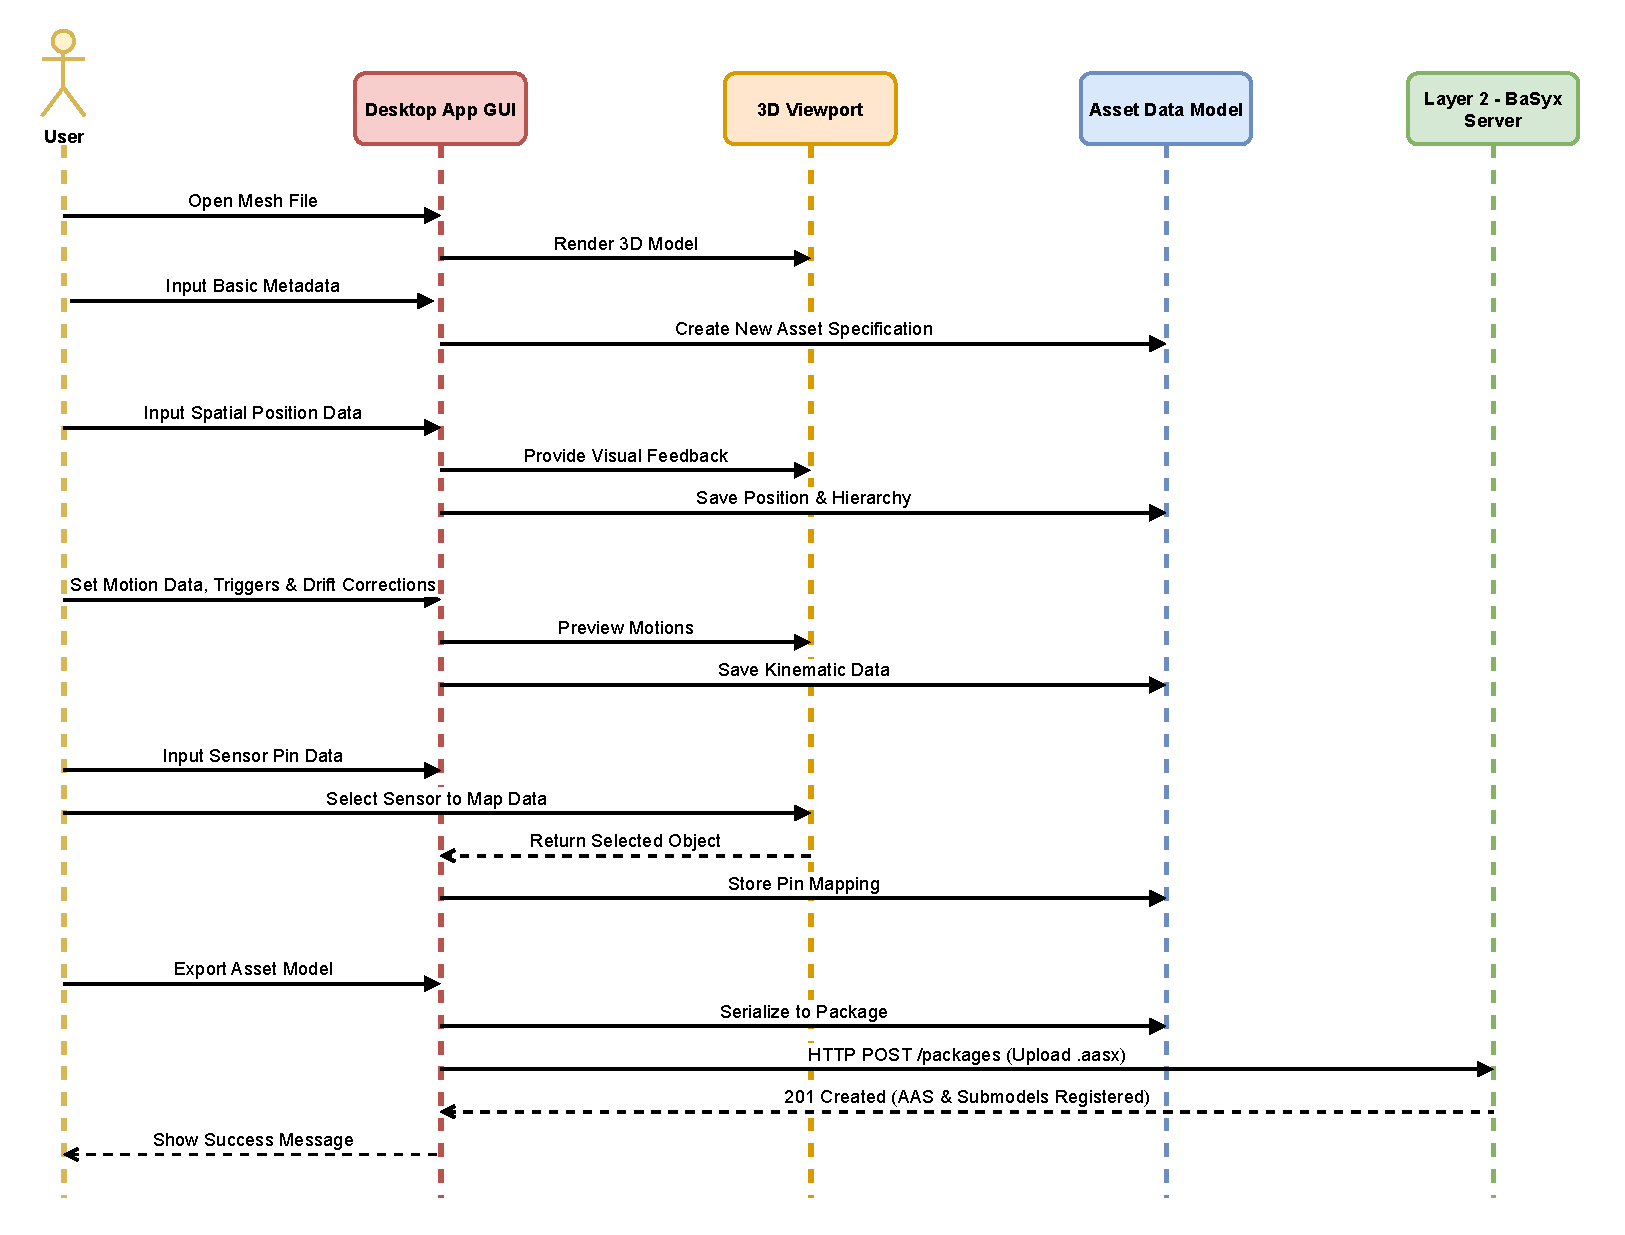
\includegraphics[width=\linewidth,height=0.72\textheight,keepaspectratio]{5-Figures/sequence_layer1.drawio.pdf}
    \caption{\gls{UML} Sequence Diagram of the Layer 1 interactive asset modeling workflow.}
    \label{fig:wizard_ui}
\end{figure}

\subsection{Integrated Rule Editor for Control Logic}
To support standalone validation during \gls{VC}, the tool includes a no-code \textit{ControlLogic} rule editor (\textbf{NFR4}). This interface lets domain engineers build sequence logic without writing code, using condition-action pairs tied to sensor states and actuator commands (\Cref{fig:rule_editor_ui}).

\begin{figure}[htbp]
    \centering
    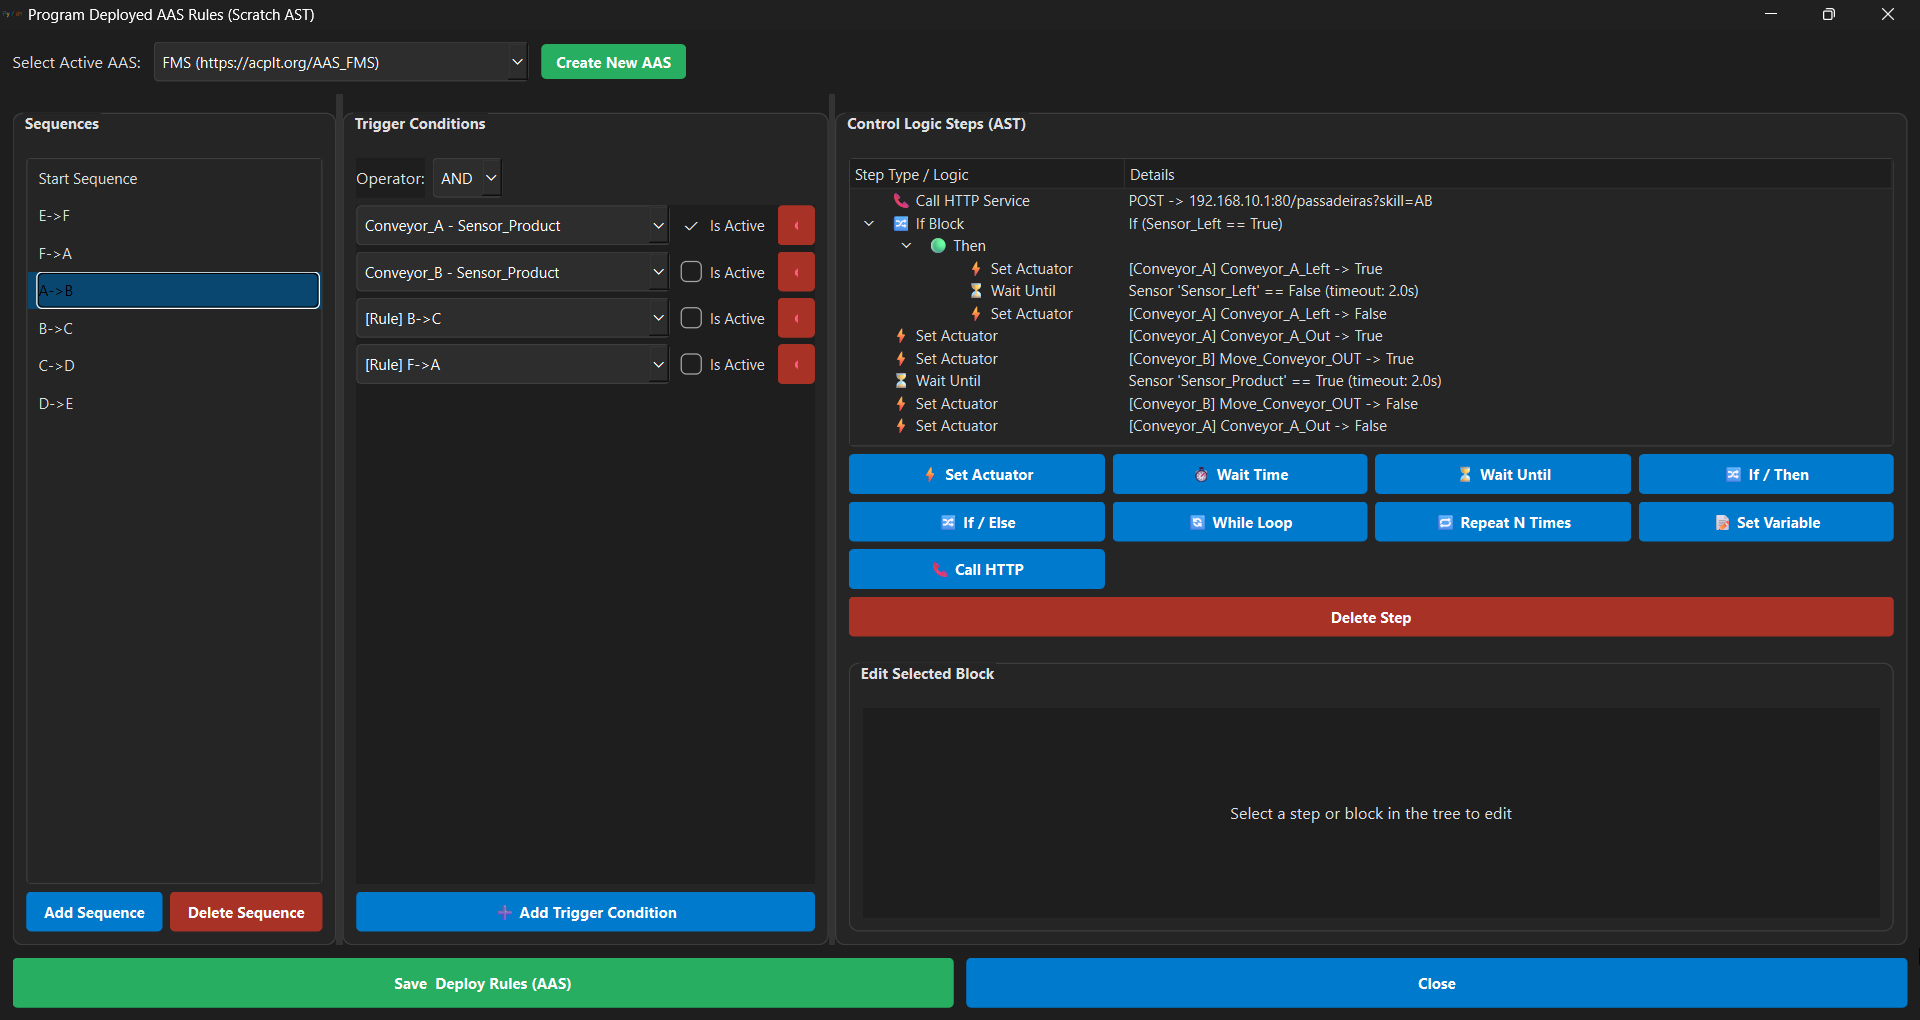
\includegraphics[width=\textwidth,keepaspectratio]{5-Figures/rule_editor_gui.png}
    \caption{\gls{UI} of the no-code \textit{ControlLogic} rule editor.}
    \label{fig:rule_editor_ui}
\end{figure}

The editor provides nine modular block types to build the logic tree:
\begin{itemize}
    \item \textbf{Set Actuator:} Changes the state of an actuator pin or motor relay.
    \item \textbf{Wait Time:} Pauses execution for a set number of seconds before continuing.
    \item \textbf{Wait Until:} Holds execution until a sensor condition is met.
    \item \textbf{If / Then:} Evaluates a condition and runs nested steps when true.
    \item \textbf{If / Else:} Provides two execution branches based on a boolean condition.
    \item \textbf{While Loop:} Repeats a group of steps while a sensor condition holds true.
    \item \textbf{Repeat N Times:} Executes a sequence for a fixed number of cycles ($N$).
    \item \textbf{Set Variable:} Updates an internal variable used across conditional checks.
    \item \textbf{Call \gls{HTTP}:} Sends an outbound \gls{HTTP} \gls{REST} request to trigger external actions or services.
\end{itemize}

These rules are saved as structured \glspl{AST} in the \textit{ControlLogic} submodel, enabling Unity's local rule engine to simulate machine sequences without an external \gls{PLC}. The \gls{UML} Sequence Diagram in \Cref{fig:sequence_rules} illustrates the rule configuration and deployment workflow.

\begin{figure}[htbp]
    \centering
    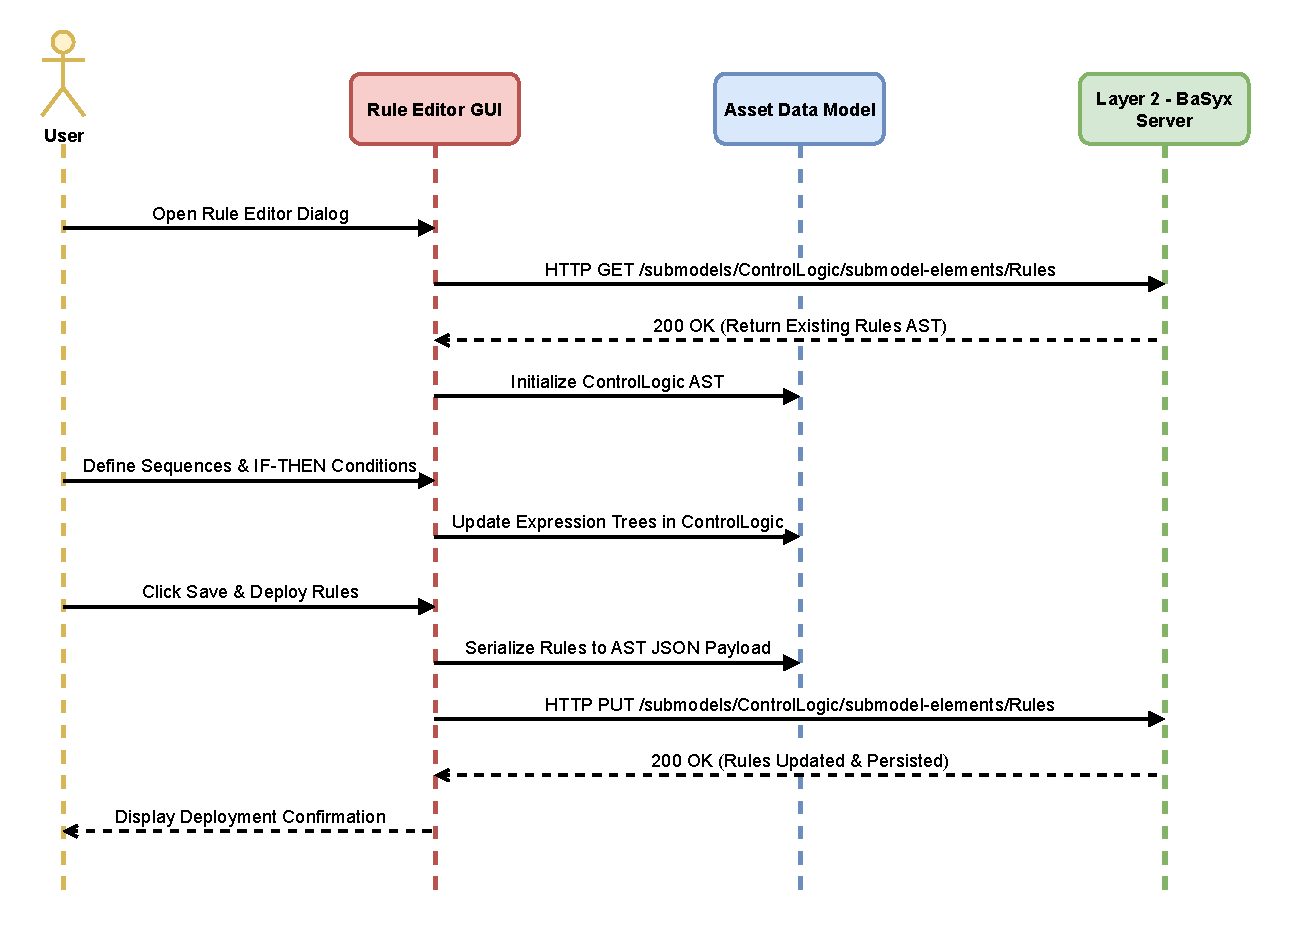
\includegraphics[width=\linewidth,height=0.72\textheight,keepaspectratio]{5-Figures/sequence_rules.drawio.pdf}
    \caption{\gls{UML} Sequence Diagram of the \textit{ControlLogic} rule configuration and deployment workflow.}
    \label{fig:sequence_rules}
\end{figure}

Once asset properties, kinematic mappings, virtual pins, and control logic are fully defined, the application initiates the export pipeline. Using the basyx-python-sdk library, the tool builds the official \gls{IEC}~63278 \gls{AASX} archive in memory. The 3D \gls{GLB} mesh is stored as an embedded binary \textit{Blob}, while the five submodels are serialized into standard-compliant \gls{JSON} manifests within the package. Finally, the application validates package integrity and automatically uploads the generated \gls{AASX} bundle to the Layer~2 BaSyx repository via \gls{REST} endpoints.

\section{Layer 2: Storage and Registry (Eclipse BaSyx v2)}
\label{sec:impl_basyx}

Layer~2 is implemented using Eclipse BaSyx~v2 deployed with Docker Compose. Docker makes the entire server stack reproducible: running Docker Compose starts all services in the right order without manual configuration. This setup allows new asset submodels and services to start automatically, fulfilling requirement \textbf{FR1} (Plug-and-Play Asset Onboarding).

The \gls{UML} Component Diagram in \Cref{fig:component_layer2} illustrates the component structure of Layer~2 (Storage and Registry), which consists of five main elements. The \gls{AAS} Environment Repository stores uploaded \gls{AASX} packages, handles package ingestion, and serves models to Unity clients. The \gls{AAS} Registry and Submodel Registry keep track of registered shells and submodel URLs, offering endpoints for registration and discovery. A shared MongoDB database stores metadata and descriptors persistently. Finally, operators can inspect active assets and submodels using the BaSyx Web \gls{GUI}.

\begin{figure}[htbp]
    \centering
    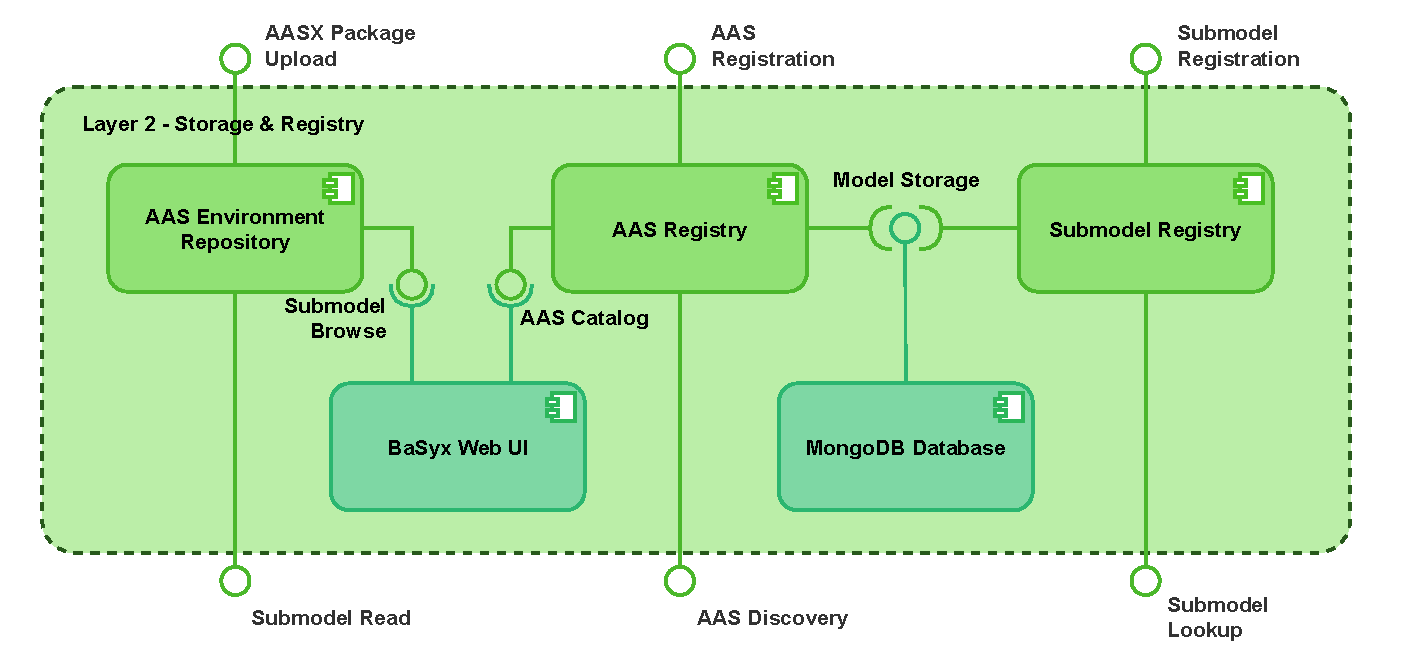
\includegraphics[width=\linewidth,height=0.72\textheight,keepaspectratio]{5-Figures/Layer 2 - Storage & Registry.pdf}
    \caption{\gls{UML} Component Diagram of Layer 2 (Storage and Registry).}
    \label{fig:component_layer2}
\end{figure}

The \gls{UML} Deployment Diagram in \Cref{fig:basyx_docker_topology} illustrates the container networking, execution environments, and service deployment topology of Eclipse BaSyx~v2.

\begin{figure}[htbp]
    \centering
    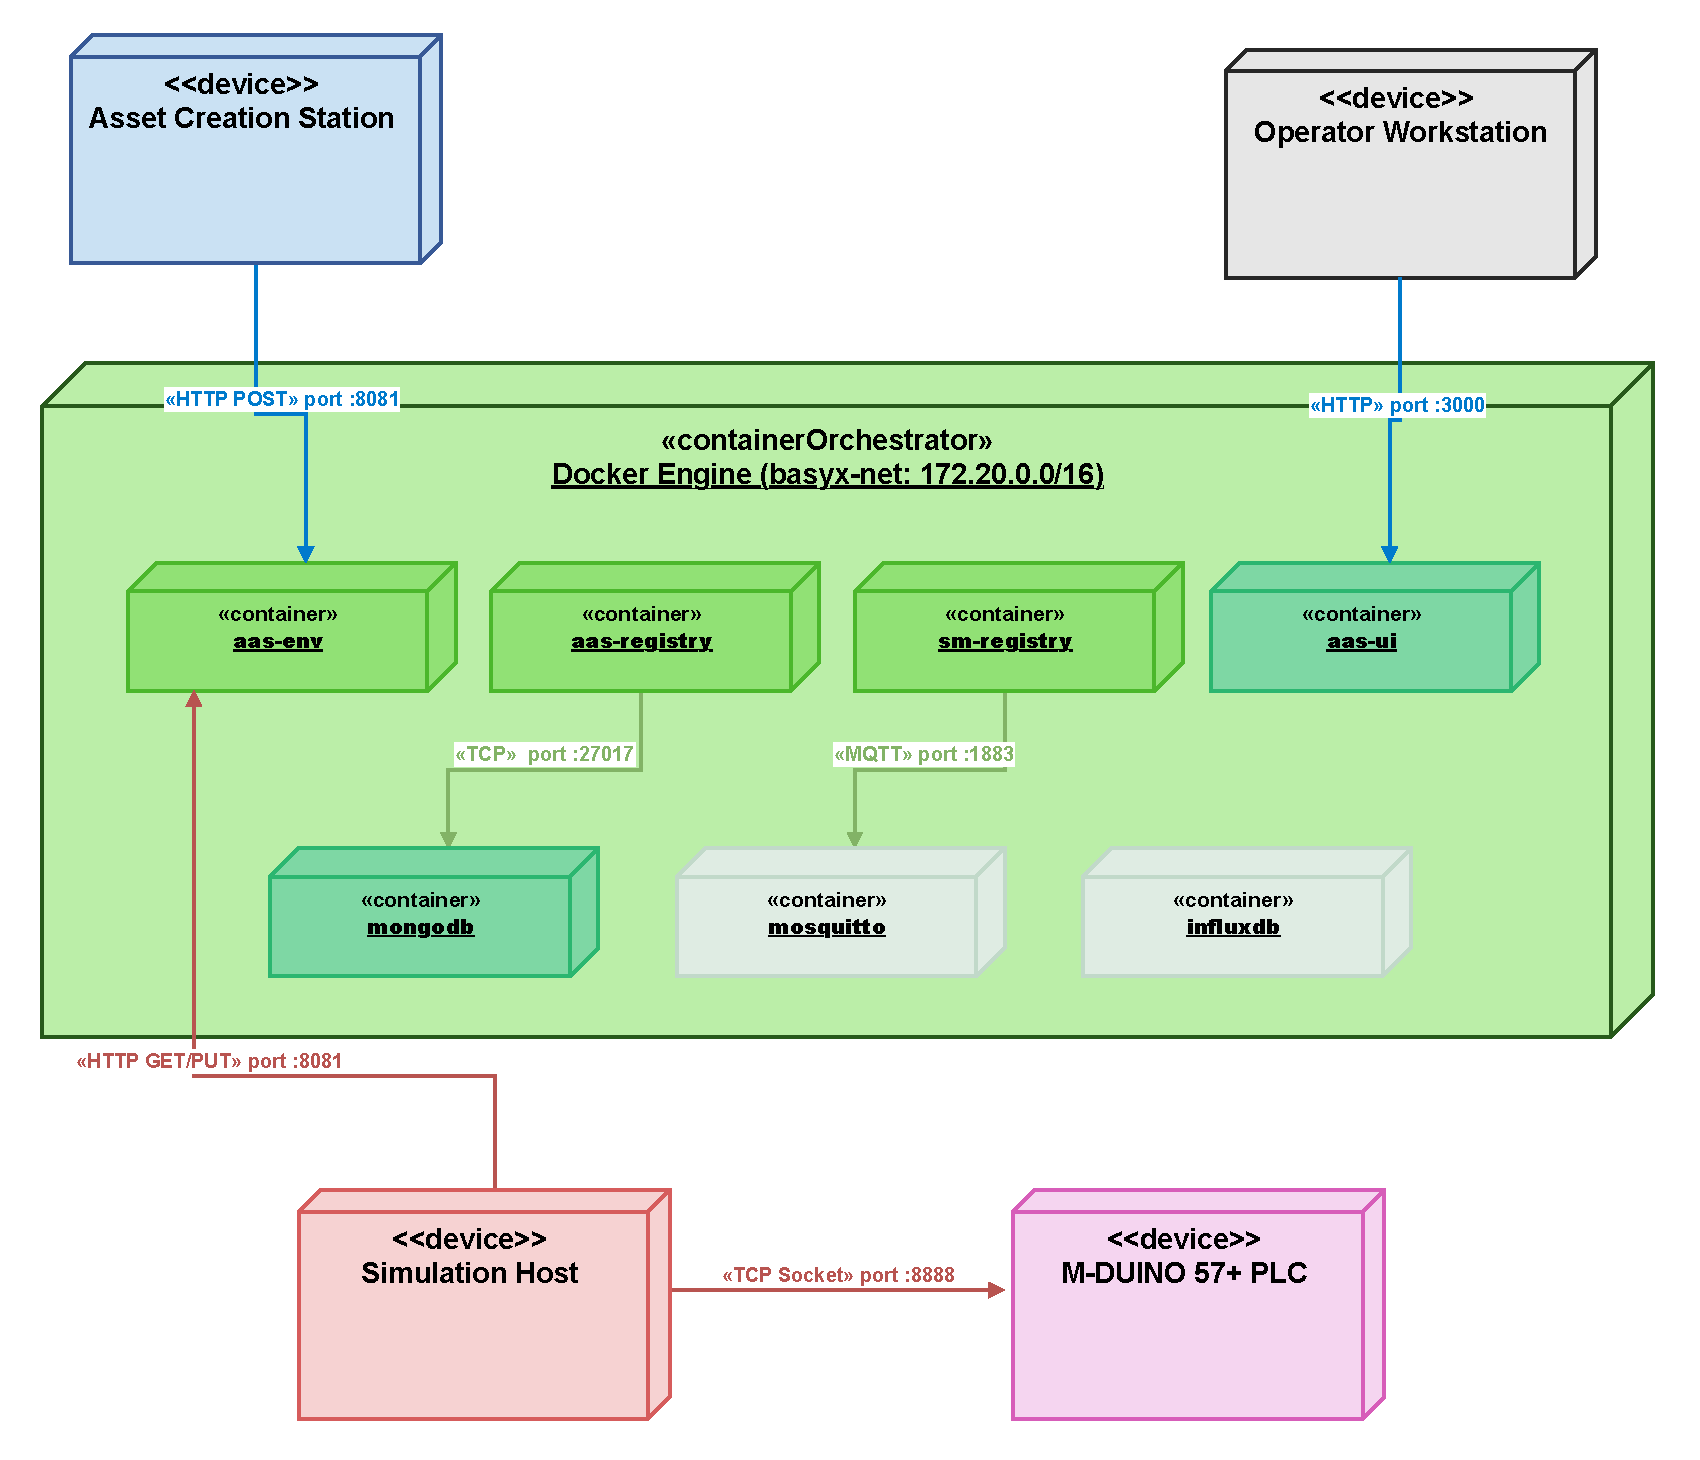
\includegraphics[width=0.85\linewidth,height=0.72\textheight,keepaspectratio]{drawio/basyx_docker_topology.drawio.pdf}
    \caption{\gls{UML} Deployment Diagram of the Eclipse BaSyx v2 Docker deployment and container topology.}
    \label{fig:basyx_docker_topology}
\end{figure}

\subsection{Microservice Architecture and Port Allocation}
The containerized services carry out the repository and registry tasks described in \Cref{fig:activity_layer2} (\cpageref{fig:activity_layer2}). The \gls{AAS} Environment Repository (port 8081) exposes standard \gls{REST} endpoints to store and serve packages, submodels, and 3D mesh files. The \gls{AAS} Registry (port 8082) and Submodel Registry (port 8083) maintain directories of active assets, mapping unique IDs to network URLs. Persistent storage is provided by MongoDB (port 27017). By separating these functions into microservices, Layer~2 scales easily as more machines and clients join the network, satisfying requirement \textbf{NFR2} (Scalability). Although the standard BaSyx stack includes Mosquitto \gls{MQTT} (port 1883) and InfluxDB (port 8086), operational \gls{DT} execution in this work uses direct \gls{TCP} sockets with the \gls{PLC} to minimize telemetry delay. Operators can inspect the running system through the BaSyx Web dashboard (port 3000).

\subsection{Package Ingestion and Registry Resolution}
When an \gls{AASX} package is uploaded via \gls{HTTP} POST to the repository endpoint (port 8081), the server decompresses the package archive and parses the internal manifests. Embedded 3D mesh files (.glb) are extracted and placed directly into the static web server directory, making them accessible to simulation clients via standard URLs. Concurrently, the \gls{AAS} metadata and individual submodels (visual structure, behavior mapping, virtual pins, control logic, and network endpoints) are committed to MongoDB for persistent retrieval.

Following successful ingestion, registration calls are dispatched to both the \gls{AAS} Registry (port 8082) and the Submodel Registry (port 8083). These records publish the asset identifier, human-readable name, and specific \gls{REST} endpoint URLs for each submodel. By centralizing these discovery records, simulation clients in Layer~3 can locate all active machines, query their physical configurations, and retrieve their operational parameters with a single directory request.

\section{Layer 3: Runtime Execution and Physical Synchronization}
\label{sec:impl_unity}

Layer~3 connects the Unity 3D simulation with the physical testbed through the components shown in the \gls{UML} Component Diagram (\Cref{fig:component_layer3}). The main orchestrator queries Layer~2 to download models and instantiate virtual assets. The asset importer parses submodel descriptors and attaches runtime scripts to the corresponding game objects. Virtual sensor inputs and actuator commands are managed by dedicated controllers, while the rule engine executes local conditional logic during \gls{VC}. The dynamic product controller handles workpiece movement and applies position corrections. Runtime modes are managed by the operation mode manager, while the hardware telemetry link streams data over \gls{TCP} and triggers physical actions via \gls{HTTP}. On the physical bench, the Industrial Shields M-DUINO \gls{PLC} reads sensor inputs through optocouplers and drives relay outputs for conveyor motors. This modular design isolates failures between layers, fulfilling requirement \textbf{NFR3} (Layer Independence).

\begin{figure}[htbp]
    \centering
    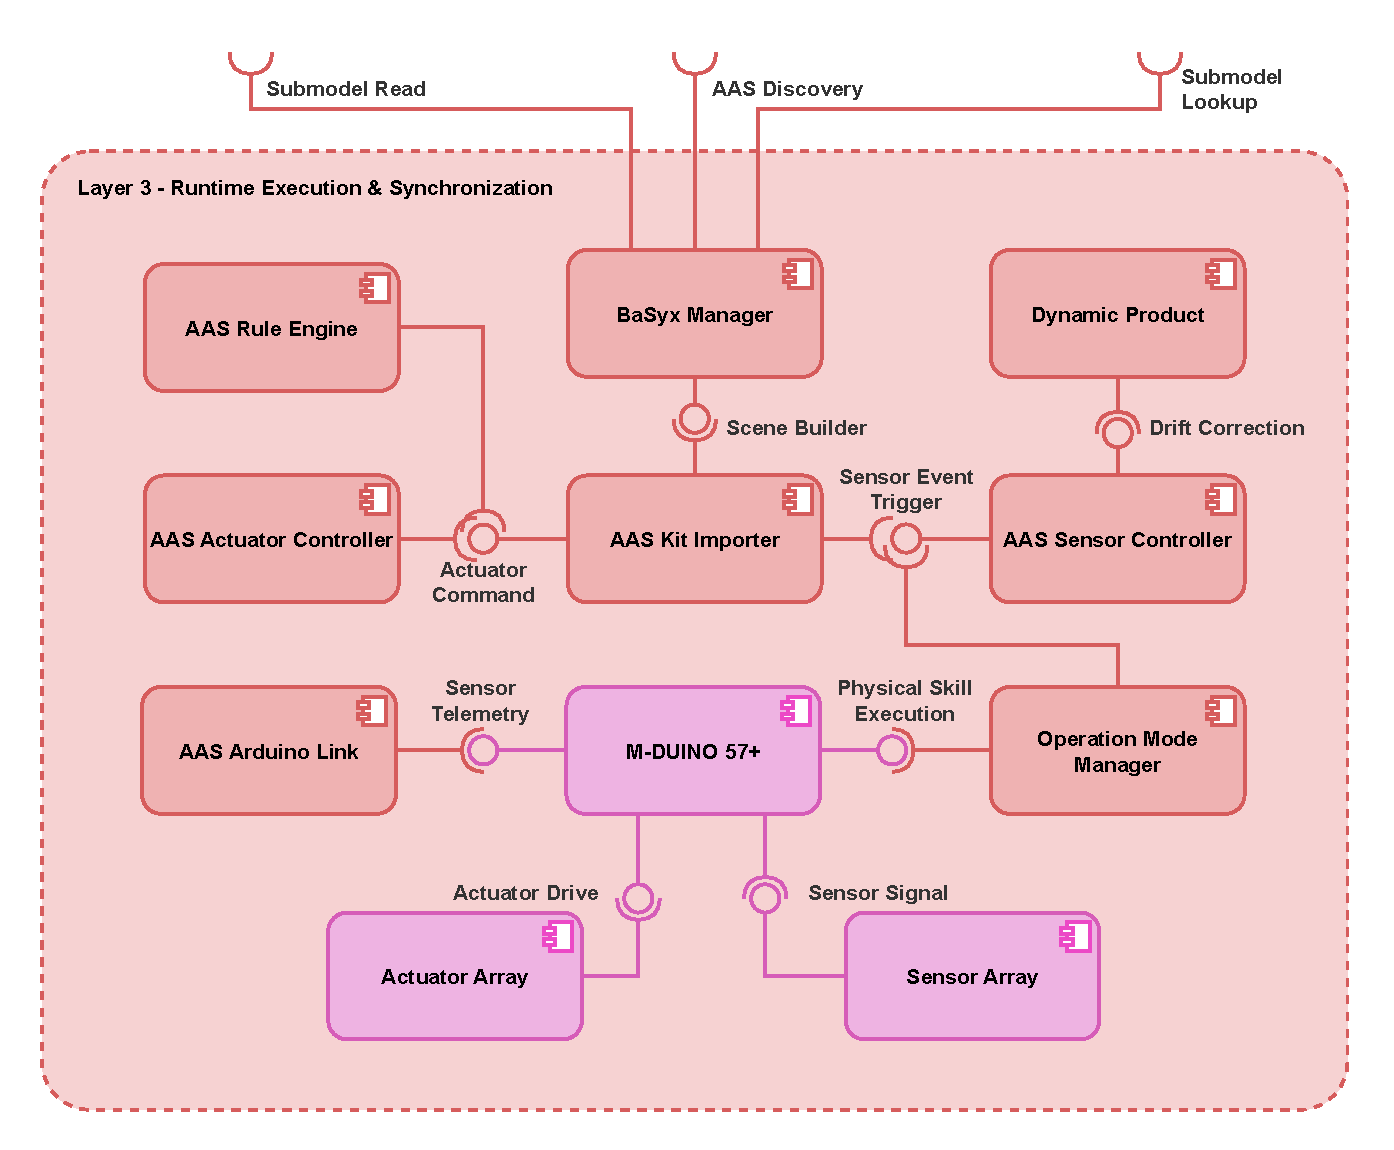
\includegraphics[width=\linewidth,height=0.72\textheight,keepaspectratio]{5-Figures/Layer 3 - Runtime Execution & Synchronization.pdf}
    \caption{\gls{UML} Component Diagram of Layer 3 (Runtime Execution and Physical Synchronization).}
    \label{fig:component_layer3}
\end{figure}

\subsection{Dynamic Ingestion Flow and Procedural Scene Construction}
To satisfy requirements \textbf{FR3} (Dynamic Scene Assembly) and \textbf{FR1} (Plug-and-Play Asset Onboarding), the Unity environment builds the scene procedurally at launch without using pre-saved scene files. The sequence follows three main phases, illustrated in the \gls{UML} Sequence Diagram (\Cref{fig:unity_runtime_sequence}):

\begin{enumerate}
    \item \textbf{Phase 1: Registry Discovery and Cache Clearing.} At launch, the orchestrator clears old cached files from disk. It then sends an \gls{HTTP} GET request to the BaSyx \gls{AAS} Registry on port 8082 to retrieve all registered assets and starts an asynchronous ingestion task for each asset found.
    \item \textbf{Phase 2: Procedural Import, Mesh Setup, and Physics Configuration.} For each asset, the importer fetches the submodels (visual structure, virtual pins, behavior mapping, and control logic) from port 8081, along with the 3D \gls{GLB} file. Using glTFast, Unity builds the 3D object hierarchy. A $180^\circ$ rotation around the Y-axis aligns Blender's right-handed coordinates with Unity's left-handed space. Non-uniform scales are applied directly to vertices to prevent distortion, and sensor/actuator scripts are attached to the corresponding nodes.
    \item \textbf{Phase 3: Dual-Mode Execution and Telemetry Loop.} After a brief settling time for physics dynamics, the runtime enters one of two operating modes:
    \begin{itemize}
        \item \textbf{Mode A (\gls{VC}):} The rule engine parses the IF-THEN rules from the control logic submodel. When a workpiece enters a sensor collider, the sensor controller notifies the rule engine, which evaluates the logic and commands virtual actuators in a closed software loop.
        \item \textbf{Mode B (\gls{DT}):} Local rule evaluation is disabled. The telemetry link opens a multi-threaded \gls{TCP} connection to the physical \gls{PLC} on port 8888. Incoming telemetry packets are placed in a queue and processed on Unity's main thread to update sensor highlights and trigger kinematic position snapping. Meanwhile, asynchronous \gls{HTTP} calls update live values in the BaSyx repository.
    \end{itemize}
\end{enumerate}

\subsection{Conveyor Physics Mechanics, Dual-Mode Execution, and Drift Correction}
\label{subsec:unity_runtime_physics}

To provide realistic behavior, conveyor belts are simulated using contact physics rather than artificial coordinate translation. Belt surfaces are configured with PhysX friction coefficients and surface speeds. When workpieces contact the belt, friction, acceleration, and contact forces are simulated naturally.

The runtime supports two execution modes (\Cref{fig:unity_runtime_sequence}):
\begin{itemize}
    \item \textbf{Mode A (\gls{VC}):} In \gls{VC} mode (\texttt{DIGITAL\_TWIN = false}), logic is tested without physical hardware. When a workpiece triggers a virtual sensor, the sensor controller informs the rule engine, which executes the IF-THEN rules from the \textit{ControlLogic} submodel to command virtual actuators.
    \item \textbf{Mode B (\gls{DT}):} In \gls{DT} mode (\texttt{DIGITAL\_TWIN = true}), local rule evaluation is disabled. The system connects directly to the \gls{PLC} via a low-latency \gls{TCP} socket (port 8888). Sensor state changes from the bench immediately update virtual markers and notify the dynamic product controller. At the same time, asynchronous \gls{HTTP} calls update live properties in the BaSyx repository.
\end{itemize}

\begin{figure}[htbp]
    \centering
    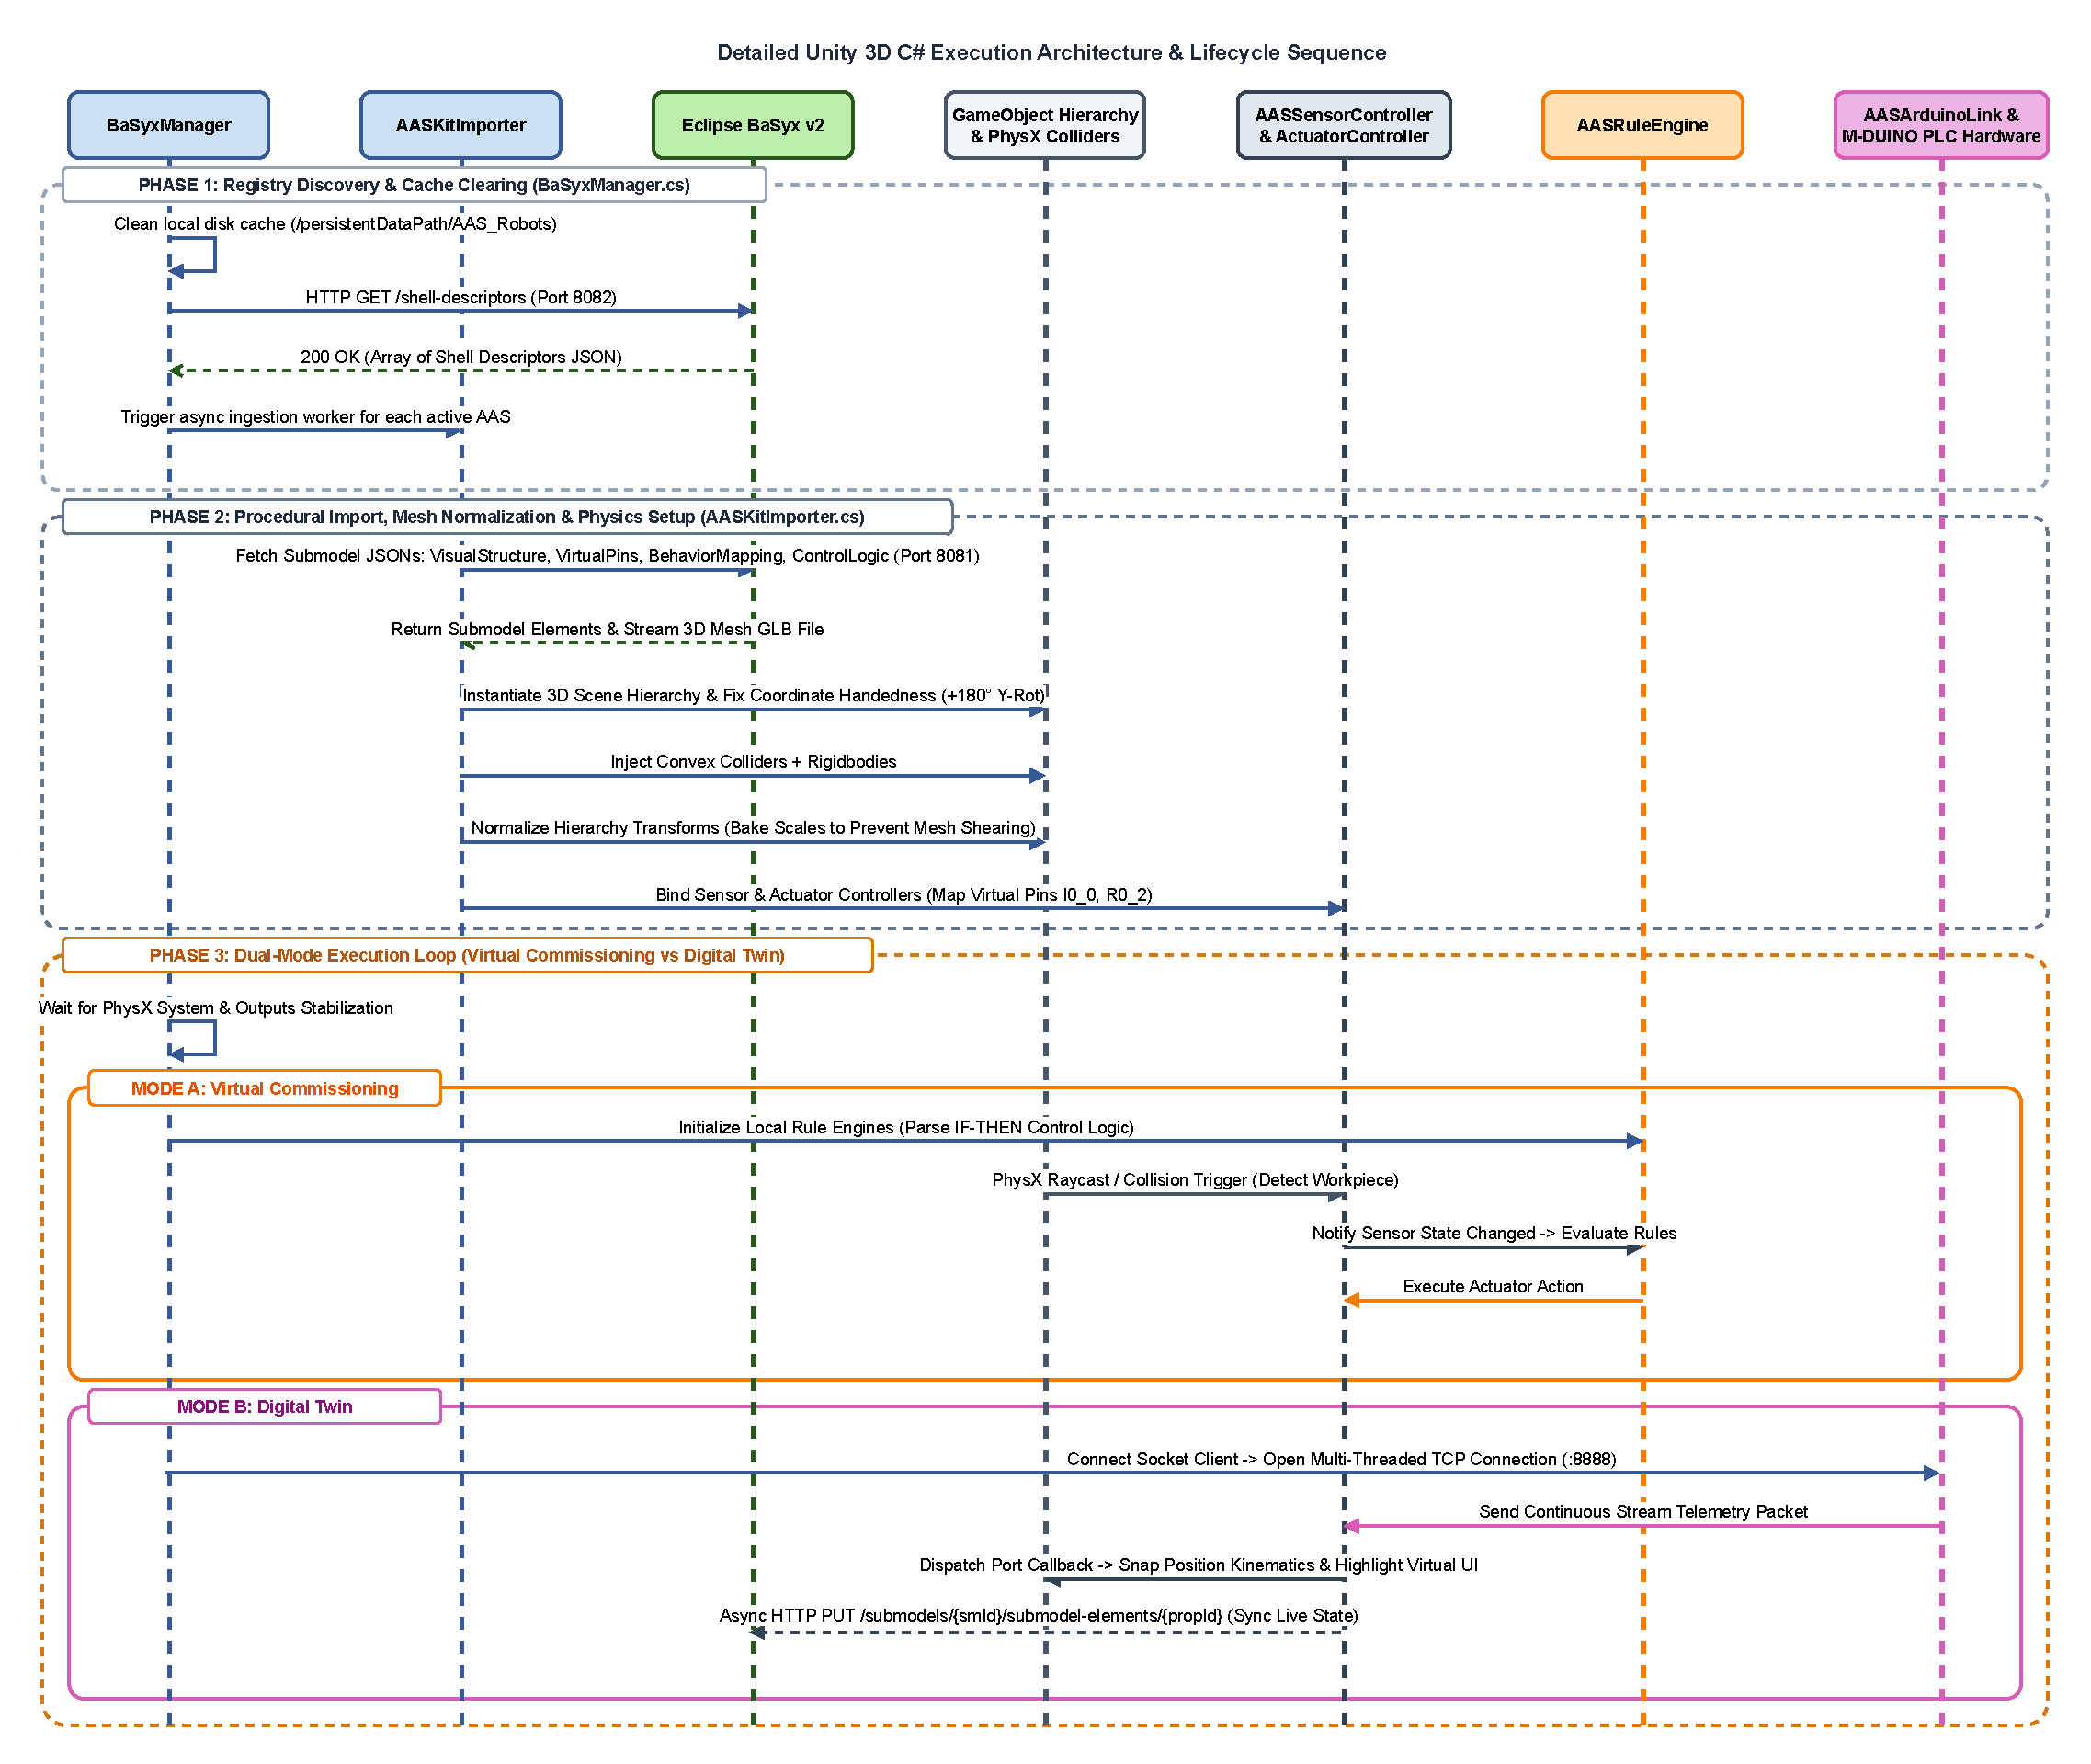
\includegraphics[width=\linewidth,height=0.75\textheight,keepaspectratio]{5-Figures/unity_runtime_sequence.pdf}
    \caption{\gls{UML} Sequence Diagram of the Unity 3D runtime execution environment.}
    \label{fig:unity_runtime_sequence}
\end{figure}

Because numerical physics calculations and network timing introduce small variations over time, virtual workpieces can drift slightly from physical parts. To meet requirement \textbf{FR4} (Physical-Virtual Synchronization), the runtime uses a kinematic snapping mechanism. When a physical sensor triggers, the runtime finds the nearest virtual workpiece and snaps its position to the known sensor coordinates, eliminating accumulated drift. \Cref{fig:unity_runtime_screenshot} shows the runtime environment running in Unity.

\begin{figure}[htbp]
    \centering
    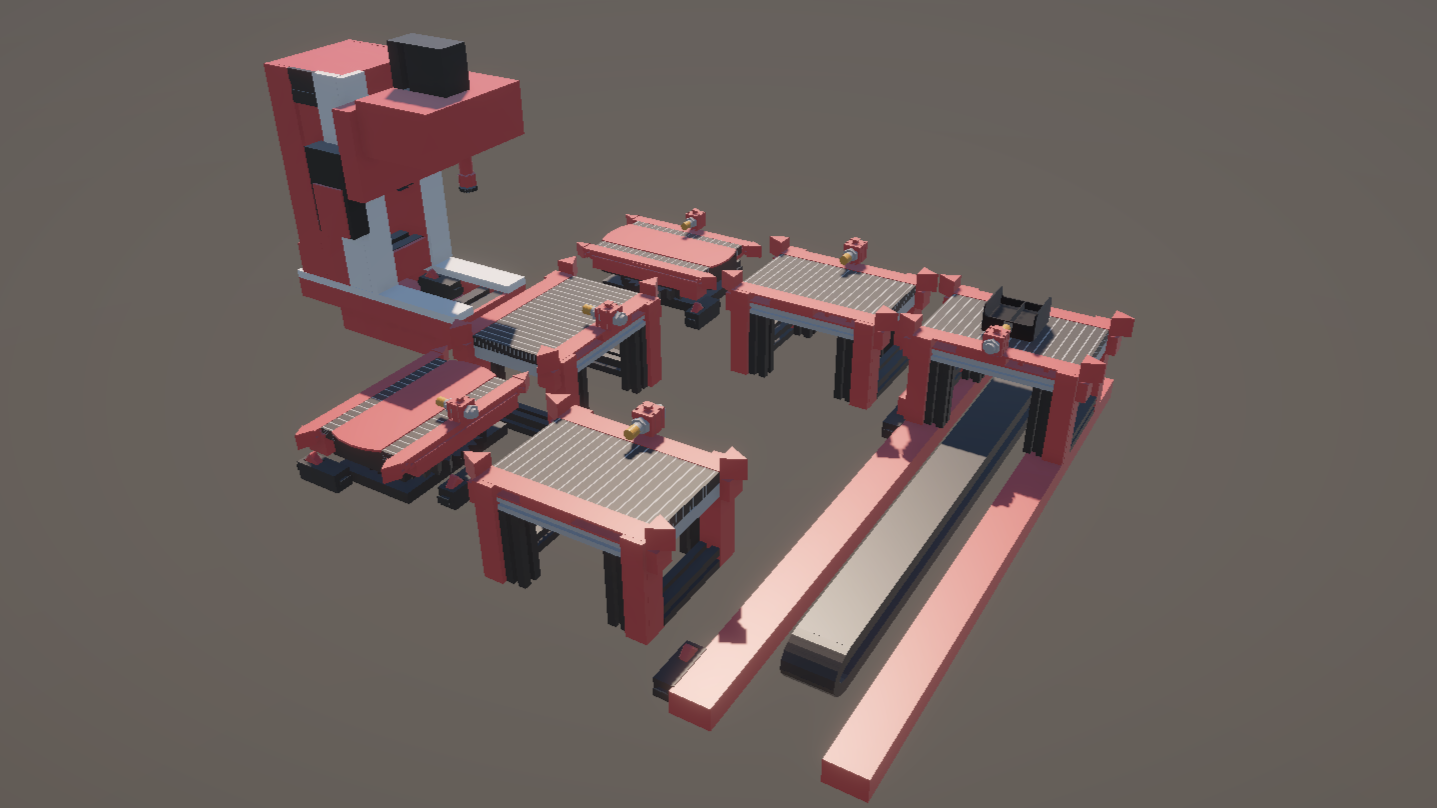
\includegraphics[width=\linewidth,keepaspectratio]{5-Figures/unity_runtime_screenshot.png}
    \caption{3D visualization and \gls{DT} runtime running in Unity 3D.}
    \label{fig:unity_runtime_screenshot}
\end{figure}

\section{Physical Automation Setup and Embedded Firmware}
\label{sec:impl_firmware}
\label{subsec:firmware_architecture}

The physical testbed is a modular closed-loop conveyor system controlled by an Industrial Shields M-DUINO 57R+ \gls{PLC}, powered by an Arduino Mega 2560 microcontroller and a W5500 Ethernet controller. The \gls{UML} Sequence Diagram in \Cref{fig:arduino_freertos_schema} illustrates the embedded FreeRTOS firmware execution across hardware setup, sensor scanning, event queues, \gls{TCP} telemetry streaming, and \gls{HTTP} actuation channels.

\begin{figure}[htbp]
    \centering
    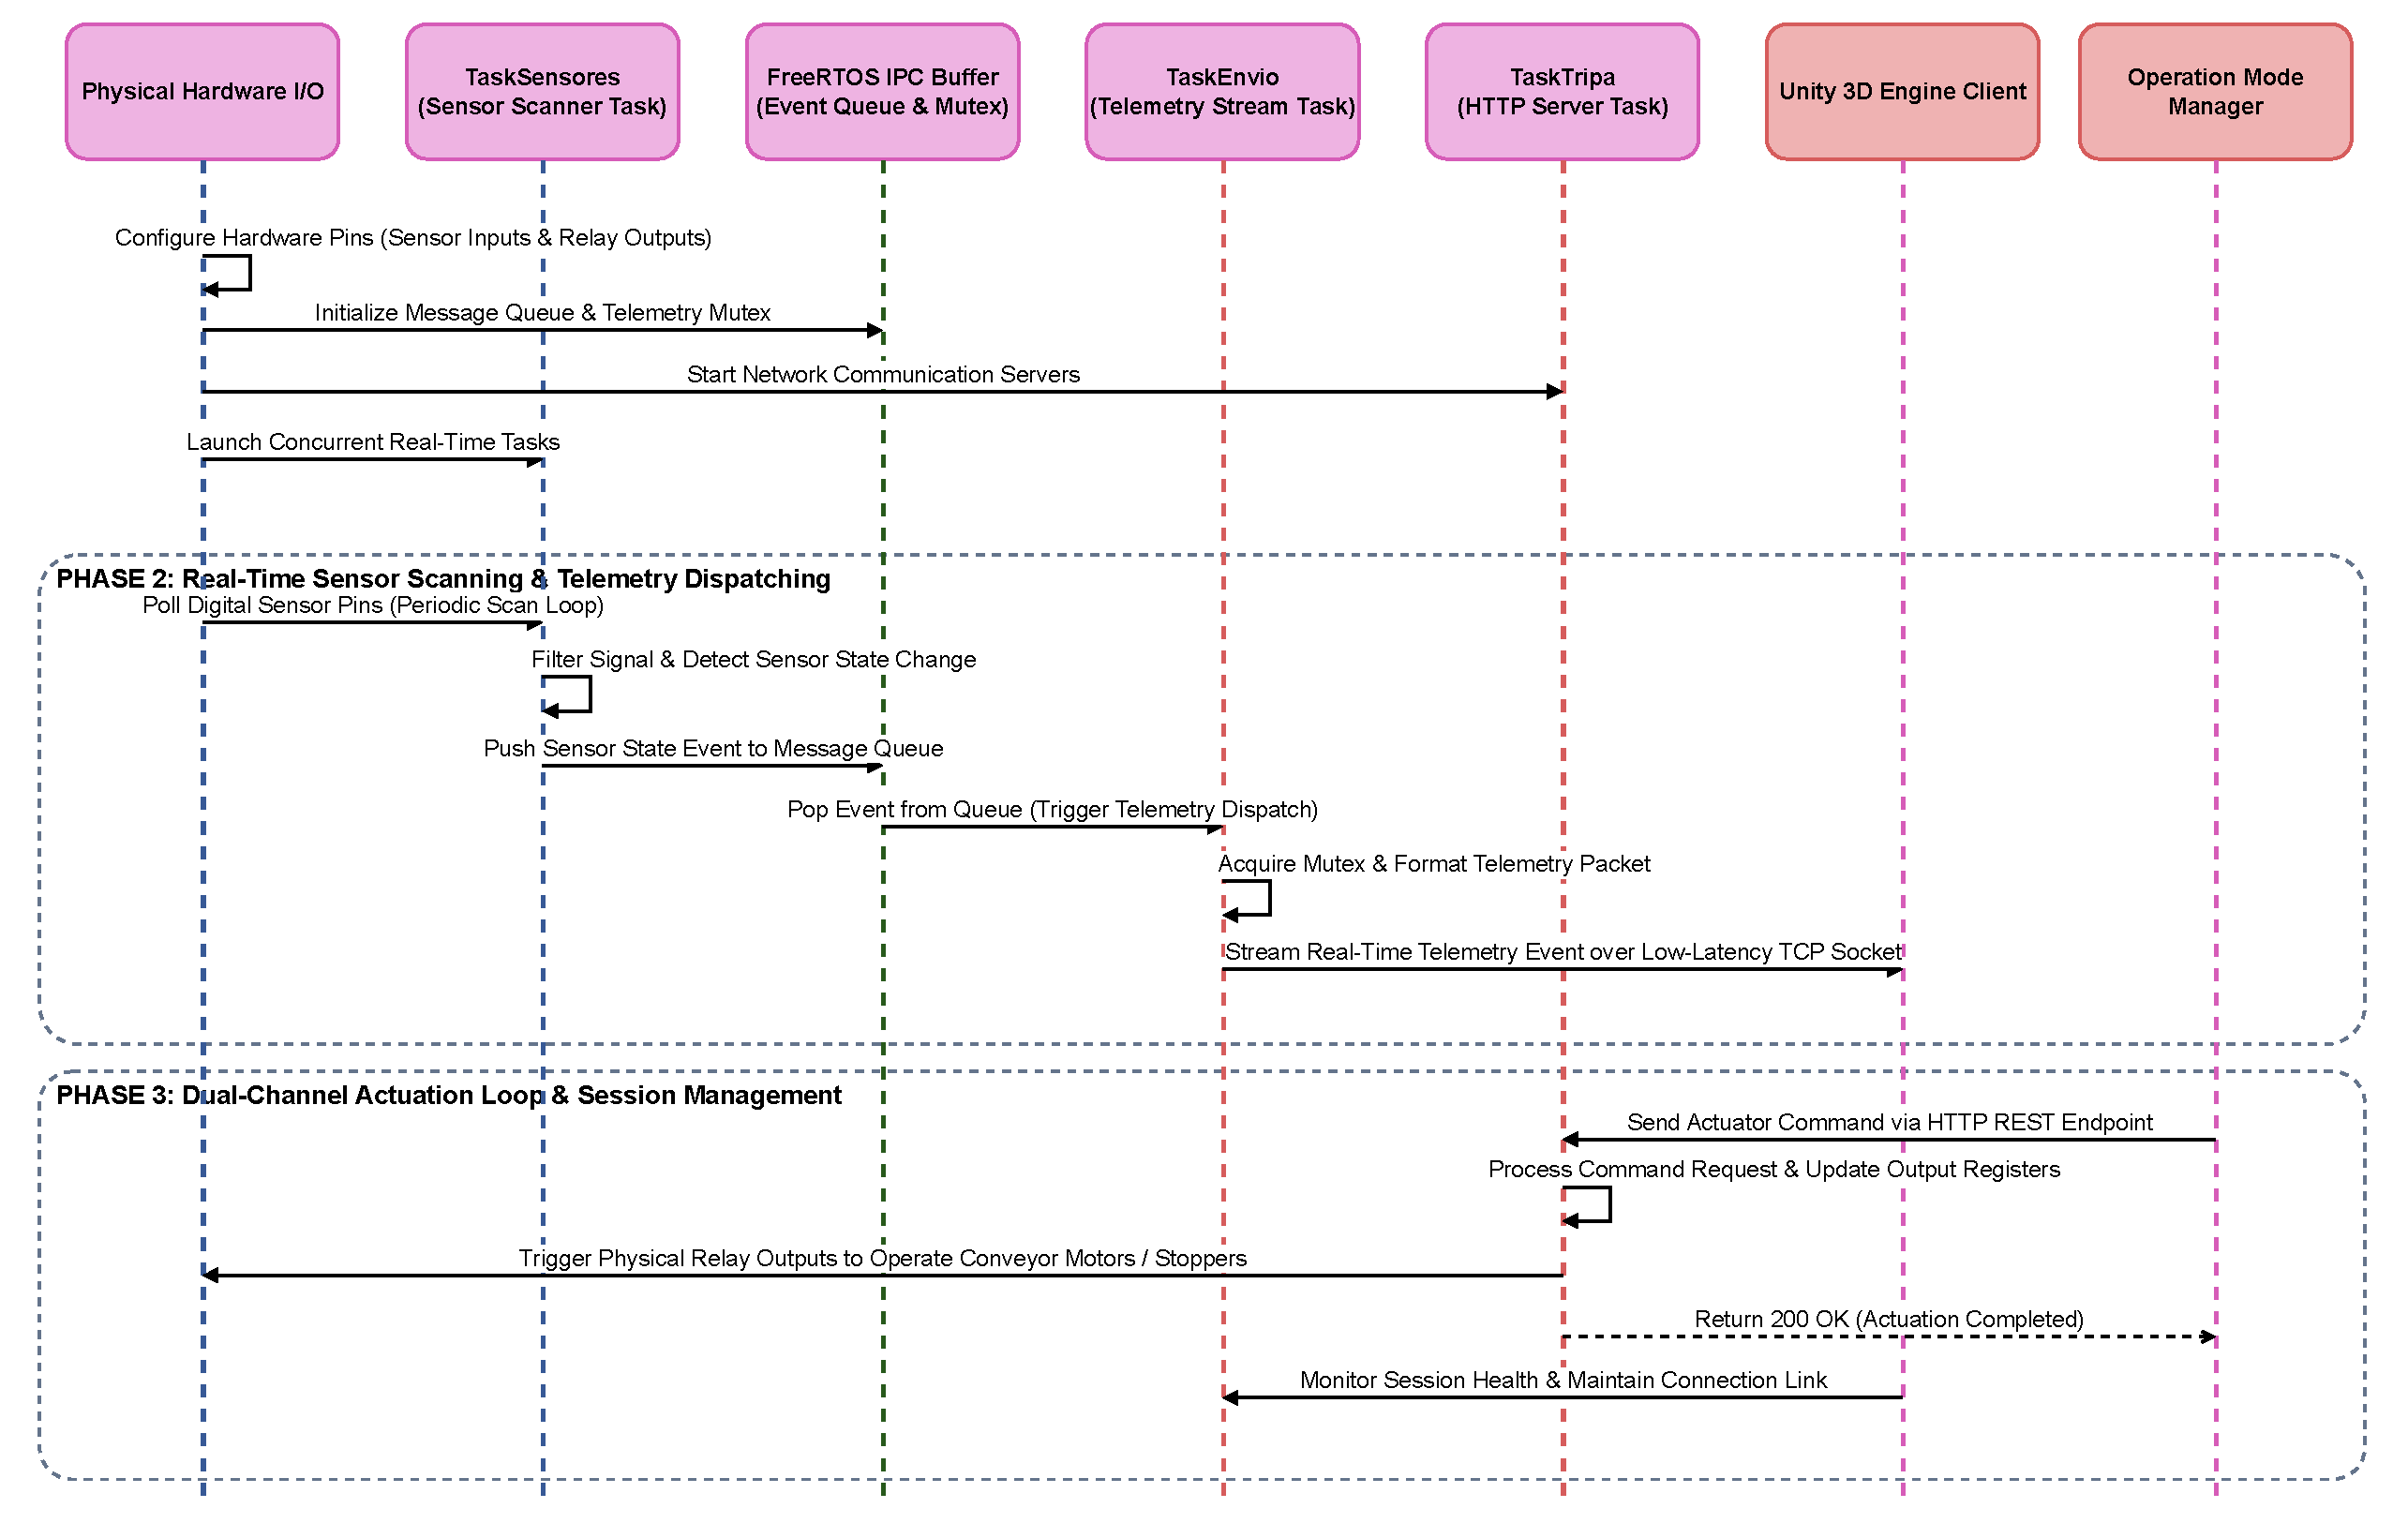
\includegraphics[width=\linewidth,height=0.72\textheight,keepaspectratio]{5-Figures/arduino_freertos_sequence.drawio.pdf}
    \caption{\gls{UML} Sequence Diagram of the embedded FreeRTOS firmware execution.}
    \label{fig:arduino_freertos_schema}
\end{figure}

The physical testbed is instrumented with 24\,V~DC magnetic sensors that detect workpieces along the tracks and push-button limit switches that detect the end positions of the moving conveyors and the punch. To protect the 5\,V microcontroller logic from electrical noise and voltage transients caused by motor switching, all field inputs pass through optocoupled galvanic isolation stages before routing to controller \gls{GPIO} pins.

The embedded firmware runs on the FreeRTOS real-time operating system to guarantee deterministic task scheduling and non-blocking network communication across four concurrent tasks:
\begin{enumerate}
    \item \textbf{Hardware Setup and Server Initialization:} On boot, the microcontroller configures input pins and motor relay output registers, initializes a 30-element \gls{FIFO} sensor event queue, and creates a mutex semaphore protecting socket transmission. It then starts an embedded \gls{HTTP} server on port 80 and a raw \gls{TCP} socket server on port 8888, handing task execution to the FreeRTOS preemptive scheduler.
    \item \textbf{Real-Time Scanning and Telemetry:} The sensor scanner task operates as the highest-priority routine (Priority 3). It performs a 5\,ms scan loop across digital input pins with software debounce filtering. When a valid state change occurs, an event token is placed in the \gls{FIFO} queue. Buffering up to 30 events in this queue prevents dropped edge transitions if temporary network jitter or socket congestion delays transmission. The queued token immediately wakes the telemetry task (Priority 2), which formats a compact \gls{JSON} packet and streams it over \gls{TCP} port 8888 to Unity with minimal latency, directly satisfying \textbf{NFR1} (Low-Latency Telemetry).
    \item \textbf{Actuation and Connection Management:} External actuation requests are handled by the \gls{HTTP} server task (Priority 1) on port 80, which parses incoming command parameters and drives physical relays. Concurrently, a session monitor task (Priority 1) performs connection watchdog checks, recovering automatically from network drops without interrupting automation routines.
\end{enumerate}

\section{Implementation Traceability and Requirement Coverage}
\label{sec:impl_traceability}

\Cref{tab:impl_traceability_matrix} maps each operational tier, core technology, and requirement to verify how the technical implementation fulfills the design criteria established in \Cref{sec:design_requirements}.

\Cref{sec:impl_layer0} and \Cref{sec:impl_wizard} address asset preparation and onboarding. By utilizing Blender 5.2 LTS to enforce a 1:1 metric scale, aligned pivot points, and low-polygon geometries, Layer~0 satisfies \textbf{FR2} (Graphical and Kinematic Fidelity). Layer~1 builds upon this foundation via a PyQt6/PyVista desktop application, leveraging an interactive 3D viewport for pin binding, a visual rule editor, and automated \gls{AASX} packaging to fulfill \textbf{FR1} (Modular Asset Specification), \textbf{FR2}, and \textbf{NFR4} (No-Code Configuration).

At the repository level (\Cref{sec:impl_basyx}), Layer~2 relies on containerized Eclipse BaSyx~v2 microservices deployed via Docker and backed by MongoDB. By maintaining decoupled \gls{AAS} and submodel registries accessible through standard \gls{REST} \gls{API} endpoints, Layer~2 satisfies \textbf{FR1}, \textbf{FR3} (Dynamic Scene Assembly), \textbf{NFR2} (Interoperability), and \textbf{NFR3} (Extensibility and Scalability). 

Finally, the execution loop is closed across Layer~3 and the physical hardware (\Cref{sec:impl_unity}, \Cref{sec:impl_firmware}). Unity 3D queries BaSyx registries at startup to perform procedural scene assembly, satisfying \textbf{FR1}, \textbf{FR3}, and \textbf{NFR3}. During runtime, PhysX contact mechanics and kinematic position snapping enforce \textbf{FR4} (Physical-Virtual Synchronization) by eliminating spatial drift between physical workpieces and virtual models. On the physical bench, the Industrial Shields \gls{PLC} running FreeRTOS delivers 5\,ms input scanning with software debouncing and dedicated \gls{TCP}/\gls{HTTP} socket streaming, directly fulfilling \textbf{NFR1} (Low-Latency Telemetry) and \textbf{FR4}.

\begin{landscape}
\vspace*{\fill}
\begin{table}[htbp]
    \centering
    \caption{Traceability matrix mapping architectural layers and technical components to design requirements.}
    \label{tab:impl_traceability_matrix}
    \small
    \renewcommand{\arraystretch}{1.4}
    \setlength{\tabcolsep}{8pt}
    \begin{tabularx}{\linewidth}{@{}p{4.0cm} p{5.5cm} p{2.8cm} X@{}}
        \toprule
        \textbf{Layer / Component} & \textbf{Core Technologies} & \textbf{Requirements} & \textbf{Functional Role} \\ \midrule
        \textbf{Layer 0: Digitization} & Blender 5.2 LTS, \gls{glTF}/\gls{GLB} & FR2 & 1:1 metric modeling, pivot alignment, low-poly geometry \\ \addlinespace[4pt]
        \textbf{Layer 1: Modeling App} & Python, PyQt6, PyVista, basyx-python-sdk & FR1, FR2, NFR4 & 3D pin binding to model nodes, rule editor, \gls{AASX} packaging \\ \addlinespace[4pt]
        \textbf{Layer 2: Storage \& Reg.} & Eclipse BaSyx v2, Docker, MongoDB, \gls{REST} & FR1, FR3, NFR2, NFR3 & Decoupled \gls{AAS} and submodel registries, dynamic asset discovery \\ \addlinespace[4pt]
        \textbf{Layer 3: Unity Runtime} & Unity 3D, C\#, glTFast, PhysX & FR1, FR3, FR4, NFR3 & Procedural scene assembly, contact physics, dual-mode execution, drift correction \\ \addlinespace[4pt]
        \textbf{Hardware \& Firmware} & Industrial Shields \gls{PLC}, FreeRTOS, \gls{TCP}/\gls{IP} & FR4, NFR1 & Fast 5\,ms input scanning, optocoupled isolation, dual-channel communication \\ \bottomrule
    \end{tabularx}
\end{table}
\vspace*{\fill}
\end{landscape}

\section{Chapter Summary}
\label{sec:impl_summary}

This chapter presented the physical and software realization of the \gls{DT} framework across four tiers. Layer~0 digitized existing conveyor hardware in Blender to produce low-poly \gls{GLB} models with properly aligned motion pivots. Layer~1 implemented the Python desktop application, enabling engineers to visually instrument equipment in a 3D viewport and generate standardized \gls{AASX} packages without programming. Layer~2 realized model storage and discovery registries using containerized Eclipse BaSyx~v2 microservices on Docker backed by MongoDB. Finally, Layer~3 implemented the runtime in Unity 3D, providing procedural scene assembly, PhysX contact mechanics, dual-mode execution (\gls{VC} and operational \gls{DT}), and drift correction. The experimental evaluation of this implementation is presented in \Cref{cha:discussion}.

